\documentclass[paper=a4,fontsize=12pt,parskip=half]{scrartcl}

\usepackage{ucs}
\usepackage[utf8x]{inputenc}
\usepackage[T1]{fontenc}
\usepackage{graphicx}
\usepackage{titlesec}
\usepackage{listings}
\usepackage{setspace}
\usepackage{xcolor}
\usepackage{color}
\usepackage{pgf}
\usepackage{enumitem}
\usepackage[ngerman]{babel}
\usepackage[autostyle=true,german=quotes]{csquotes}
\usepackage[acronym,hyperfirst=false]{glossaries}
\usepackage[colorlinks]{hyperref}
\usepackage{acronym}
\usepackage[colorinlistoftodos,prependcaption]{todonotes}
\usepackage{soul}
\usepackage{subcaption}
\usepackage{hyperref}
\hypersetup{
	colorlinks=true,% make the links colored
}

% Besseres highlighting von Worten
% https://tex.stackexchange.com/questions/343458/
\makeatletter
\if@todonotes@disabled
\newcommand{\hlnote}[2]{#1}
\else
\newcommand{\hlnote}[2]{\todo{#2}\texthl{#1}}
\fi
\makeatother

\titlespacing*{\section} {0pt}{0ex}{0ex}
\titlespacing*{\subsection} {0pt}{0ex}{0ex}
\titlespacing*{\subsubsection} {0pt}{0ex}{0ex}

\lstdefinestyle{CodeView} {
	columns=flexible,
	numbers=left,
	basicstyle=\footnotesize,
	tabsize=4,
	frame=single,
	backgroundcolor=\color{white},
	keywordstyle=\color{blue},
}

\colorlet{punct}{red!60!black}
\definecolor{background}{HTML}{EEEEEE}
\definecolor{delim}{RGB}{20,105,176}
\colorlet{numb}{magenta!60!black}

\lstdefinelanguage{JavaScript}{
	keywords={typeof, new, true, false, catch, function, return, null, catch, switch, var, if, in, while, do, else, case, break},
	keywordstyle=\color{blue}\bfseries,
	ndkeywords={class, export, boolean, throw, implements, import, this},
	ndkeywordstyle=\color{darkgray}\bfseries,
	identifierstyle=\color{black},
	sensitive=false,
	comment=[l]{//},
	morecomment=[s]{/*}{*/},
	commentstyle=\color{purple}\ttfamily,
	stringstyle=\color{red}\ttfamily,
	morestring=[b]',
	morestring=[b]"
}


\lstdefinelanguage{JSON}{
	basicstyle=\normalfont\ttfamily,
	numbers=left,
	numberstyle=\scriptsize,
	stepnumber=1,
	numbersep=8pt,
	tabsize=4,
	showstringspaces=false,
	breaklines=true,
	frame=lines,
	backgroundcolor=\color{background},
	literate=
	*{0}{{{\color{numb}0}}}{1}
	{1}{{{\color{numb}1}}}{1}
	{2}{{{\color{numb}2}}}{1}
	{3}{{{\color{numb}3}}}{1}
	{4}{{{\color{numb}4}}}{1}
	{5}{{{\color{numb}5}}}{1}
	{6}{{{\color{numb}6}}}{1}
	{7}{{{\color{numb}7}}}{1}
	{8}{{{\color{numb}8}}}{1}
	{9}{{{\color{numb}9}}}{1}
	{:}{{{\color{punct}{:}}}}{1}
	{,}{{{\color{punct}{,}}}}{1}
	{\{}{{{\color{delim}{\{}}}}{1}
	{\}}{{{\color{delim}{\}}}}}{1}
	{[}{{{\color{delim}{[}}}}{1}
	{]}{{{\color{delim}{]}}}}{1},
}

\onehalfspacing

\title{Abschlussarbeit}
\author{Tom Hilge}

\makeglossaries

\newcommand{\JS}{JavaScript}
\newcommand{\TS}{TypeScript}

\newacronym{JWT}{JWT}{JSON Web Token}
\newacronym{URI}{URI}{Uniform Resource Identifier}
\newacronym{HTTP}{HTTP}{Hypertext Transfer Protocol}
\newacronym{CSS}{CSS}{Cascading Style Sheets}
\newacronym{JSON}{JSON}{JavaScript Object Notation}
\newacronym{MVC}{MVC}{Model View Controller}
\newacronym{HTML}{HTML}{Hypertext Markup Language}
\newacronym{DOM}{DOM}{Document Object Model}
\newacronym{SPA}{SPA}{Single Page Application}
\newacronym{CLI}{CLI}{Command Line Interface}
\newacronym{API}{API}{Application Programming Interface}
\newacronym{RFC}{RFC}{Request for Comments}
\newacronym{MIME}{MIME}{Internet Media Type}
\newacronym{HMAC}{HMAC}{Keyed-Hash Message Authentication Code}
\newacronym{SHA256}{SHA256}{Secure Hash Algorithm 256 Bit}
\newacronym{oAuth2}{oAuth2}{Open Authorization 2.0}
\newacronym{UUID}{UUID}{Universally Unique Identifier}
\newacronym{STI}{STI}{Single Table Inheritance}
\newacronym{XSS}{XSS}{Cross-Site-Scripting}
\newacronym{CSRF}{CSRF}{Cross-Site-Request-Forgery}
\newacronym{HTTPS}{HTTPS}{Hypertext Transfer Protocol Secure}
\newacronym{URL}{URL}{Uniform Resource Locator}

\begin{document}
	\hypersetup{linkcolor=black, urlcolor=black}

   	\tableofcontents
	\clearpage
	
	\section{Einleitung}

In Deutschland scheint man Informatik als eine Hochschulangelegenheit zu betrachten. Anders ist es für mich kaum zu erklären, dass der Informatikunterricht an Schulen zwar durchaus vorgesehen ist, der Begriff ``Informatik'' dabei aber oftmals sehr weit interpretiert wird. Der Umgang mit Textverarbeitung, Tabellenkalkulation und Präsentationsmitteln wird heutzutage zwar an fast jeder Schule zumindest thematisiert, Inhalte mit tatsächlichem Bezug zur Informatik wie sie in einer späteren Ausbildung oder im Studium relevant relevant wären, sind dabei aber in der Minderheit. Schaut man sich die für Informatikinhalte zur Verfügung stehenden Lehr- und Lernprogramme an (natürlich sollte Informatikunterricht auch am Rechner stattfinden!), verwundert diese stiefmütterliche Behandlung nur wenig: Die Menge an verfügbarer und gepflegter Software ist ausgesprochen überschaubar. Und natürlich ist es keinem Informatiklehrer zuzumuten, diese Lücke mit eigens geschriebener Software zu füllen.

Diese Arbeit ist ein Versuch, eine Lehrsoftware für zwei wichtige Teilgebiete der Informatik anzubieten: Datenmodellierung und (Web-)Oberflächenentwicklung. Ganz konkret geht es um die Konzeption und prototypische Implementierung einer einsteigerfreundlichen Entwicklungsumgebung für den anwendungsorientierten Umgang mit SQL-Datenbanken. Zielgruppen dieser Software sind Schülerinnen und Schüler an weiterführenden Schulen sowie natürlich deren Lehrkräfte. Die Anwender sollten mit dem prototypischen Stand der Software in die Lage versetzt werden, zu einem gegebenen Datenmodell sowohl inhaltliche Fragen mit Bezug zu einem konkreten Datenbestand zu beantworten als auch neue Daten in das Modell einzupflegen. Darüber hinaus soll es ihnen möglich sein, die Datenbank über eine selbst gestaltete Oberfläche einer begrenzten Öffentlichkeit zugänglich zu machen.

Aus praktisch Gründen sollte an dieser Stelle die Lernsoftware "`Scratch"' nicht unerwähnt bleiben: Der Arbeitstitel für die Thesis lautete "`Scratch für SQL und Webanwendungen"' und weckt bei Leuten, die mit Scratch schon vertraut sind, damit durchaus gewünschte, positive Assoziation. Wie Scratch versucht auch \idename{} viele typische und demotivierende Hürden wie Syntaxfehler, komplexe Entwicklungsumgebungen oder kryptische Fehlermeldungen konstruktiv auszuschließen. Kapitel \ref{sec:related-work}~"`\nameref{sec:related-work}"' beschreibt neben Scratch noch weitere, einflußreiche Inspirationsquellen.

Der wesentliche Anspruch an die im Rahmen dieser Arbeit zu erstellende Software ergibt sich also sowohl aus dem Titel der Arbeit als auch der Arbeitsweise von Scratch: Es geht vorrangig um die Vermittlung von praktischen Kenntnissen zur Abfrage, Manipulation und Visualisierung von komplexen Datenbeständen in Anlehnung an die Projektideen der Lehrpläne \cite{lehrplan-inf-sek-1} bzw. Fachanforderungen \cite{lehrplan-inf-sek-2} für Informatik des Landes Schleswig-Holstein\footnote{Die exakte Verortung im Curriculum oder auch die Konzeption von konkreten Schulstunden ist hingegen nicht Teil dieser Arbeit.}. Auch wenn sich aktuell eine zunehmende Pluralität von Paradigmen zur Datenspeicherung abzeichnet, welche das relationale Modell ergänzen oder in Frage stellen, behandelt diese Arbeit explizit die Vermittlung von SQL-Kenntnissen. Die Visualisierung erfolgt dabei über HTML-Seiten, welche sich von den unterschiedlichsten Endgeräten abrufen lassen.

Das Kapitel \ref{sec:requirements}~"`\nameref{sec:requirements}"' analysiert auf Basis der vergleichbaren Arbeiten und unter Berücksichtigung eigener Ideen, wie eine solche "`praktische"' Lernsoftware für datengetriebene Anwendungen aussehen könnte. Da sich die dort gesammelten Funktionen nicht alle in dem für die Thesis zur Verfügung stehenden Zeitrahmen umsetzen lassen, ist das softwaretechnische Ergebnis dieser Thesis als ein "`minimum viable product"' zu verstehen. Die Umsetzung dieses Prototypen wird in Kapitel \ref{sec:implementation-analysis}~"`\nameref{sec:implementation-analysis}"' beschrieben.



%%% Local Variables:
%%% mode: latex
%%% TeX-master: "thesis"
%%% End:

	\section{Technologien}
\label{sec:technology}
Im Verlauf dieser Sektion werden die Technologien\todo{Warum diese?} und deren Verwendungszweck
kurz erläutert.

\subsection{Blattwerkzeug}
\label{sec:blattwerkzeug}
Blattwerkzeug ist ein quelloffenes Projekt, dass Informatik-Interessierten das Programmieren von zum Beispiel \gls{HTML} Grundgerüsten und SQL\todo{kein gls?} Statements per \enquote{drag and drop} näher bringen kann. Dabei versteckt Blattwerkzeug die Syntax nicht vor dem Nutzer, sondern gibt ihm die Möglichkeit diesen gleich mit einzusehen. Dadurch wird es möglich, in einer ``richtigen'' Programmiersprache zu entwickeln, ohne sich von Beginn an mit syntaktischen Details beschäftigen zu müssen.

\begin{figure}[h]
	
\includegraphics[scale=0.6]{graphics/blattwerkzeug.png}
\end{figure}

\subsection{Passwort Hashing}
\label{sec:password_hashing}

Sobald eine Software mit Nutzerdaten geführt wird, ergibt sich das Problem des Speicherns der Passwörter der jeweiligen Nutzer.
Denn sollten die Daten der Nutzer im Klartext in der Datenbank gespeichert werden und ein Angreifer erlangt Zugriff auf die Datenbank, so ist es für ihn ein leichtes weitere Konten der Nutzer zu infiltrieren. Der Grund dafür sind die anwendungsübergreifenden, vom Nutzer grö{\ss}tenteils identischen, Passwörter.

\begin{figure}[h]
	\centering
	\includegraphics[width=\textwidth]{graphics/example-plaintext-password.pdf}
	\caption{Beispiel einer Infiltrierung bei Klartext Passwort.}
\end{figure}

\todo[inline]{Vorsicht, der Angriff erlaubt nicht das entschlüsseln des Passworts bei Gmail, es erlaubt nur den Login (sofern das gleiche Passwort verwendet wurde. Vielleicht stattdessen lieber exemplarisch mehrere Anbieter zeigen?}

An diesem Punkt kommt das Hashen von Passwörtern zum Einsatz. Passwort Hashing soll dem Nutzer Sicherheit gewährleisten und es einem Angreifer nicht möglich machen mit erlangten Daten weitere Konten der Nutzer zu infiltrieren. Dabei wird aus einem Passwort ein Hash generiert. Dieser Hash macht es einem unmöglich, das Passwort wiederherzustellen. Jedoch ergibt sich bei gleicher Eingabe, der gleiche Hash. Um ein gehashtes Passwort zu erhalten, muss ein Hashing Algorithmus auf das jeweilige Klartext Passwort angewendet werden.

\begin{figure}
	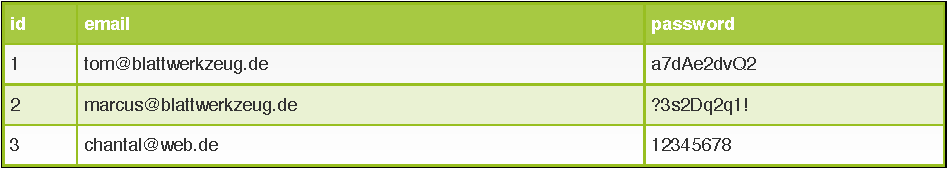
\includegraphics[width=\textwidth]{graphics/unhashed_table.pdf}
	\caption{Tabelle mit ungehashten Passwörtern}
	\label{fig:unhashed_table}
\end{figure}

\begin{figure}
	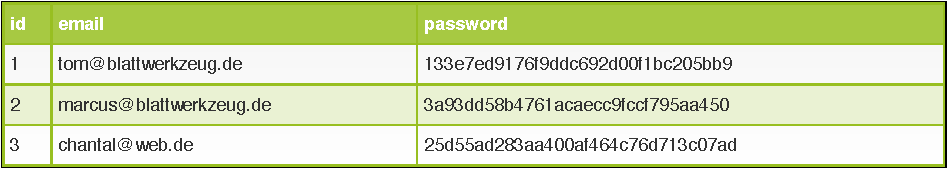
\includegraphics[width=\textwidth]{graphics/md5_table.pdf}
	\caption{Tabelle mit MD5 gehashten Passwörtern}
	\label{fig:md5_hashed_table}
\end{figure}

\begin{figure}
	\includegraphics[width=\textwidth]{graphics/salted_table.pdf}
	\caption{Tabelle mit Salting Hashes}
	\label{fig:salted_table}
\end{figure}

\begin{figure}
	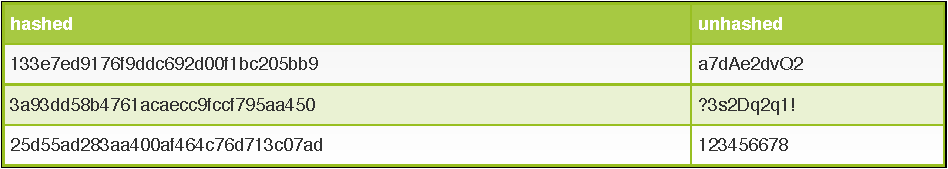
\includegraphics[width=\textwidth]{graphics/rainbowtable.pdf}
	\caption{Beispiel einer Rainbowtable.}
	\label{fig:rainbowtable}
\end{figure}

Mittlerweile gibt es eine vielzahl an Hashfunktionen, von denen manche als nicht mehr sicher gelten. Der Grund dafür sind Rainbowtables in denen Hashes mit dazugehörigem Klartext Passwort (Abbildung \ref{fig:unhashed_table}) stehen. Das Nutzen einer nicht sicheren Hashfunktion stellt ein Sicherheitsrisiko dar, da die Möglichkeit besteht, das gehashte Passwort mit einer Rainbowtable (Abbildung \ref{fig:rainbowtable}) abzugleichen und dabei das jeweilige Klartext Passwort zu erhalten. Aus diesem Grund werden MD5 (Abbildung \ref{fig:md5_hashed_table}) und SHA zwei der bekanntesten Hashfunktionen, seit geraumer Zeit nicht mehr zum Passwort hashen verwendet werden. Ein Beispiel für eine derzeitig nutzbare Hashfunktion ist bcrypt. Bcrypt bietet den Vorteil des Integrierten Saltings. (Abbildung \ref{fig:salted_table})

Salts (Abbildung ~\ref{fig:salted-hash}) sind zufällig generierte Zeichenketten, die dem Klartext-Passwort hinzugefügt werden. Der zusammengesetzte String wird mittels Hashfunktion verschlüsselt.

\begin{figure}
	\centering
	\includegraphics[width=.7\textwidth]{graphics/salting.pdf}
	\caption{Hashfunktion auf Klartext und Salt angewandt.}
	\label{fig:salted-hash}
\end{figure}

\subsection{Sessions}
\label{sec: sessions}
Das \gls{HTTP} ist ein zustandsloses Protokoll, dass sich\todo{Wort zuviel?} keine Informationen der jeweiligen Aufrufe zwischenspeichert. Das hat den Vorteil, dass ohne jegliche Vorbedingung eine vielzahl an Verbrauchern auf eine Anwendung zugreifen kann. Die Zustandslosigkeit ist allerdings dann unpraktisch, wenn Daten eines Benutzer kurzeitig gespeichert werden sollen. Ein Verwendungszweck wäre beispielsweise der Warenkorb, da dieser nur temporär vorhanden sein soll.

Die Session ist eine serverseitige Daten-Speichermöglichkeit. Dabei wird bei der Anfrage von einem Client an den Server ohne Session-ID eine Session und Session-ID erstellt. Diese Session-ID wird bei der Antwort des Servers mit an den Client ausgeliefert. Ab diesem Punkt wird bei jeder Anfrage vom Client an den Server die Session-ID mit gesendet. Dies kann über einen Cookie oder über die \gls{URI} erfolgen. Aufgrund dessen kann der Server dem Client Daten aus der jeweiligen Session zur Verfügung stellen.

Eine weitere Möglichkeit Daten zwischenzeitig zu speichern sind Cookies. Cookies werden clientseitig gespeichert und häufig für das Aufbewahren der Session-ID verwendet. Desweiteren werden Cookies ebenfalls verwendet um Warenkörbe zu realisieren. Ein Problem hierbei ist die Vertrauenswürdigkeit eines Cookies, da dieser beliebig modifiziert werden kann.

\subsection{JSON Web Token}
\label{sec: jwt}
\enquote{\gls{JWT} sind auf \gls{JSON} basierende \gls{RFC} 7519 genormte Access-Token.}\todo{Warum langes Zitat?} \gls{RFC} ist eine Sammlung aus Dokumenten, in denen das Verhalten der Technologien des Internets beschrieben ist. Einige davon gehören zum Standard und werden somit in den meisten Fällen vorausgesetzt. In speziellen Fällen möchte beispielsweise ein Unternehmen eigene Protokolle verwenden, die nicht zum Standard gehören.

Diese Tokens werden zur eindeutigen Identifizierung von Nutzern verwendet und können die Session ersetzen. Dabei ist es bei einem \gls{JWT} nicht vonnöten\todo{Mehr: Nicht vorgesehen} die Daten auf dem Server zu speichern. Dies hat zur Folge, dass die Pflege des Speichers an diesem Punkt entfällt. Jedoch haben \gls{JWT}s einen gro{\ss}en Nachteil, denn sobald der Server einen \gls{JWT} ausgestellt hat, ist dieser bis zum Ablauf des Tokens gültig. Das hei{\ss}t, sollte ein Server die Berechtigung eines Nutzers nach Ausstellung eines \gls{JWT} ändern, ist diese Änderung erst bei erneutem Erstellen eines \gls{JWT} gültig.

Ein \gls{JWT} besteht aus Header, Payload und Signatur. Dabei ist der Header und die Payload jeweils ein \gls{JSON} Objekt.

\subsubsection{Header}
\label{sec: jwt_header}

\todo[inline]{Welche Art von Daten kommen in den Header?}

\begin{description}
	\leftskip=1em
	\item[typ] Der typ Claim beschreibt den \gls{MIME} des \gls{JWT}, dieser wiederum teilt dem Client oder Server mit, um welche Art von Medium an Daten es sich handelt. Der Standardwert dieses Claims beläuft sich auf \enquote{JWT}, übersetzt \enquote{application/jwt}.
	\item[alg] Der alg Claim beschreibt die Verschlüsselungsmethode. Ein Beispiel ist \gls{HMAC} mit \gls{SHA256}, HS256 abgekürzt.
\end{description}

\begin{figure}[h]
	\centering
	\includegraphics[width=\textwidth]{graphics/jwt-header.png}
	\caption{Beispiel eines \gls{JWT} Headers }
	\label{fig:jwt-header}
\end{figure}

\subsubsection{Payload}
\label{sec: jwt-payload}

Die Payload beinhalteten Schlüssel-Wert Paare werden Claims genannt. Dabei handelt es sich um ein JSON Objekt, bei dem bestimmte Schlüssel des Objektes bereits reserviert sind. Diese nennen sich registrierte Claims. Au{\ss}erdem gibt es öffentliche und private Claims. Hierbei wird zwischen öffentlichen und privaten differenziert.

\noindent
\textbf{Beispiel registrierter Claims}

\begin{description}
	\leftskip=1em
	\item[iss]
	Der iss Claim steht für den Austeller des Tokens, beispielsweise eine Domain.
	\item[exp] Der exp Claim kennzeichnet den \gls{JWT} mit einem Ablaufdatum.
\end{description}

\noindent
\textbf{Öffentliche Claims}

Öffentliche Claims sind zusätzlich zum Standard nutzbar und ihre Namen sollten semantisch dem dazugehörigen Wert entsprechen. Au{\ss}erdem sollten die Namen der Claims Netzwerkübergreifend verständlich sein (Listing \ref{lst:public_claim}).

\noindent
\textbf{Private Claims}

Private Claims werden nur innerhalb eines Netzwerkes verwendet. Aus diesem Grund gibt es keine implizite Beschränkung in der Namensgebung (Listing \ref{lst:private_claim}).

\begin{minipage}{\linewidth}
	\lstinputlisting[label={lst:public_claim}, language=JSON, caption=Beispiel eines Öffentlichen Claims, captionpos=b]{snippets/public_claim.json}

	\lstinputlisting[label={lst:private_claim}, language=JSON, caption=Beispiel eines Privaten Claims, captionpos=b]{snippets/private_claim.json}
\end{minipage}

\subsubsection{Signatur}
\label{sec: jwt_signature}

Um die Signatur zu erhalten muss, die Payload und der Header Base64 kodiert werden. Au{\ss}erdem müssen diese beiden kodierten Zeichenfolgen mit einem Punkt als Trennzeichen verknüpft werden. Darauffolgend wird eine Hashfunktion auf das jeweilige Ergebnis mit zusätzlich sicherer Zeichenfolge als Parameter angewandt. Da diese sichere Zeichenfolge, auch Private Key genannt, nur auf dem Server hinterlegt ist, ist es dem Client zwar möglich den \gls{JWT} zu verändern, ihn jedoch mit korrekter Signatur zu versehen nicht.\todo{Folgerung: Server erkennt Manipulation}

\subsubsection{Zusammengesetzes Token}
\label{sec: jwt_result}
Schlussendlich ergibt sich der \gls{JWT} aus kodiertem Header, kodierten Payload und der Signatur. Dabei steht der Header am Anfang (Abbildung \ref{fig:jwt-encoded}, rot gekennzeichnet). Darauffolgend mit einem Punkt getrennt die Payload und zum Schluss die Signatur, ebenfalls mit einem Punkt getrennt.

\begin{figure}[h]
	\centering
	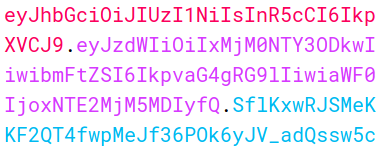
\includegraphics[width=\linewidth]{graphics/jwt-encoded.png}
	\caption{Beispiel eines kodierten \gls{JWT} }
	\label{fig:jwt-encoded}
\end{figure}

\subsection{Ruby on Rails}
\label{sec: rails}
Ruby on Rails ist ein quelloffenes Webframework für die Programmiersprache Ruby. Das Webframework nutzt das \gls{MVC} Muster und stellt bereits ein sehr umfangreiches \gls{CLI} zur Verfügung. Mittels des generate Werkzeugs kann\todo{Plural} beispielsweise Model, View und Controller erstellt werden. Jeder dieser Komponenten wird automatisch in die erstellte Rails Anwendung eingebunden. Au{/ss}erdem\todo{Typo} stellt Rails eine umfangreiche Test-Architektur und einen Service zum Versenden von Mails zur Verfügung. Dabei kann der Inhalt der E-Mail im Textformat oder als \gls{HTML} versendet werden. Einer der wesentlichen Vorteile von Ruby on Rails ist jedoch\todo{``Jedoch'' in Abgrenzung zu was?} die Datenbankanbindung. Hierbei bietet Rails einen nachhaltigen und rücksichtsvollen Umgang mit der Datenbank, zum Beispiel die Migrationen. Migrationen erlauben, die Datenbank, ohne explizite SQL-Statements, zu verändern. Zusätzlich erleichtern Migrationen die Implementierung einer Datenbankstruktur auf einem anderen System.

\subsubsection{Routen}
\label{sec: routen}
Die Routen in Rails verweisen auf einen Controller und auf eine Funktion innerhalb des Controllers. Dabei wird die Route meistens mit der Anfragemethode eingeleitet, beispielsweise \enquote{get}. Routen können in sogenannte \enquote{scopes} (Listing \ref{lst:routes_scopes}) unterteilt werden. Somit ist es nicht vonnöten bei einer verschachtelten \gls{URI} redundant zu werden (Listung \ref{lst:routes_redundant}).

\begin{minipage}{\linewidth}
	\lstinputlisting[language=Ruby, style=CodeView, caption=Beispiel einiger redundanter Routen, captionpos=b, label={lst:routes_redundant}]{snippets/routes_redundant.rb}
\end{minipage}

\begin{minipage}{\linewidth}
	\lstinputlisting[language=Ruby, style=CodeView, caption=Beispiel einiger Routen mit scope, captionpos=b, label={lst:routes_scopes}]{snippets/routes.rb}
\end{minipage}
\todo[inline]{Syntaxfehler bei Listen}


\subsubsection{Controller}
\label{sec: rails_controller}
Der Controller dient hierbei zur Kapselung von bestimmten Prozessen. Jede Route verweist in irgendeiner Weise auf eine Controller Funktion\todo{Wirklich zwei Worte?}. In der jeweiligen Controller Funktion wird dann meistens mit einem Model interagiert. Es wird beispielsweise eine Benutzerberechtigung abgefragt und individuell auf die Berechtigung reagiert. Um auf die jeweilige Berechtigung zu reagieren, gibt es mehrere Möglichkeiten. Eine der Möglichkeiten wäre, direkt ein View Template auf dem Server zu rendern und an den Client auszuliefern. Eine andere Möglichkeit wäre ein \gls{JSON} Objekt zurück zu geben und darauf mit dem Client zu agieren.

\subsubsection{Model}
\label{sec: rails_model}
Das Model in Rails stellt jeweils eine Datenbanktabelle dar\todo{nicht stellt dar, sondern ``bildet ab''}. Die Attribute des Models sind die entsprechenden Spalten der Datenbanktabelle. Jeweilige Datenbankeinträge, die über das Model erstellt werden, können mittels Validatoren auf ihre Gültigkeit geprüft werden. Diese Validatoren werden innerhalb des Models festgelegt und auf ein Attribut des Models zugewiesen. Rails bietet dabei bereits verfügbare Validatoren, zum Beispiel \enquote{presence: true}. Dieser Validator sorgt für das Vorhandensein eines Wertes ungleich \textit{nil}. Jedes Model kann zusätzliche Funktionen beinhalten, die direkt auf den jeweiligen Datenbankeintrag angewandt werden können. Ebenso bietet Rails die Möglichkeit die Beziehungen zwischen Datenbanktabellen direkt in den Modellen festzulegen.

\subsubsection{View}
\label{sec: rails_view}
Die View stellt in Rails die Möglichkeit \gls{HTML} Template auf dem Server zu rendern. Dabei kann bei dem Rendern das \gls{HTML} Template dynamisch verändert werden. Da diese Komponente während dieser Thesis keine Rolle gespielt hat, wird diese nicht weiter erläutert.

\subsubsection{Zusammenfassung}
\label{sec: rails_resuemee}
Letzendlich wird über die Route auf den jeweiligen Controller zugegriffen. Dieser fragt in den meisten Fällen nach einem bestimmten Eintrag eines Models. Darauffolgend wird mit dem Ergebnis der Anfrage interagiert. Es werden Veränderungen oder Abfragen bestimmter Daten getätigt. Danach wird ein Ergebnis dem Client ausgeliefert.

\begin{figure}[h]
	\includegraphics[width=\textwidth]{graphics/rails-mvc.pdf}
	\caption{Ablauf zwischen Client, Server, Route, Controller und Model}
	\label{fig:rails-mvc}
\end{figure}

\todo[inline]{Besser: ``BlattWerkzeug'' durch ``Routing'' ersetzen und dann den ``Rückweg'' nicht mehr dadurch führen.}

\subsection{Angular}
\label{sec: angular}
Angular ist ein TypeScript basiertes\todo{basierendes} Front-End Webframework, dass in vielen Fällen\todo{Weasel} für \gls{SPA} verwendet wird. \gls{SPA}s laden ihren Inhalt lediglich in ein einziges \gls{HTML} Dokument\todo{Abgrenzen zu klassischen Webseiten mit Links}. Der Inhalt dieses \gls{HTML} Dokumentes wird dynamisch, von beispielsweise einem Framework wie Angular, verändert. Der wesentliche Vorteil von Angular sind die klaren Entwurfsmuster. Jede Komponente in Angular hat im wesentlichen die gleiche Struktur. Dies hat zur Folge, dass Angular eine sehr gute Codekonsistenz bietet.

\subsubsection{Component}
\label{sec: ang-component}
Komponenten in Angular bieten die Möglichkeit \gls{HTML}, \gls{CSS} und TypeScript zu kapseln. Das bedeutet, dass jede Komponente unabhängig von einer anderen Komponente arbeiten kann.

\todo[inline]{Fehlt: Ein- und Ausgaben, wird im nächsten Absatz etwas merkürdig vorweggenommen. Ruhig mit sehr kleinem Codebeispiel wenn dir das bei der Erklärung hilft.}

\subsubsection{Services}
\label{sec: ang-service}
Zur Kommunikation mit einem Server und/oder zum Datenaustausch zwischen unterschiedlichen Komponenten wird meistens ein Service verwendet. Bei einem Datenaustausch zwischen Eltern- und Kind-Komponente ist es jedoch einfacher dies mittels der Kind-Komponente durchzuführen. Services werden bei dem Laden der Module instanziiert und dem Konstruktor der Komponente als instanziiertes Objekt übergeben.

\subsubsection{Module}
\label{sec: ang-modul}
Zusätzlich bietet Angular auch die Möglichkeit eigene Module zu erstellen in denen dann als Beispiel Services und Komponenten zusätzlich abgekapselt werden können. Ein Vorteil von Angular gegenüber anderen JavaScript Frameworks sind die bereits von Angular mitgelieferten Module, beispielsweise das Routing- oder das HTTP-Modul. Das Routing-Modul wird für jegliche Navigation auf der Anwendung genutzt. Das \gls{HTTP}-Modul hingegen bietet die Möglichkeit mittels jeglicher Anfragemethoden mit dem Server zu kommunizieren.

\subsection{oAuth2}
\label{sec: oauth2}
\gls{oAuth2} ist ein offenes \gls{RFC} 6749 Protokoll, welches verwendet wird, um eine Authentifizierung einer Anwendung mittels Drittanbieter zu ermöglichen. Hierbei wird der Nutzer zuerst auf die jeweilige Seite des Drittanbieters weitergeleitet. Dort muss der Nutzer sich authentifizieren und den Zugriff auf die Daten seines Kontos bestätigen. Nachdem der Zugriff auf die Daten bestätigt wurde, erhält die jeweilige Anwendung von dem Drittanbieter einen Autorisierungstoken. Dieser Autorisierungstoken wird darauffolgend von der Anwendung genutzt, um einen Zugriffstoken von dem Drittanbieter zu erhalten. Dieser ermöglicht am Ende den Zugriff auf die spezifischen Nutzerdaten des Drittanbieters. (Abbildung ~\ref{fig:oauth2})

In Blattwerkzeug wird genau dieser umfangreiche Vorgang von Omniauth übernommen. Aus diesem Grund wird oAuth2 in dieser Thesis nicht weiter erläutert.

\begin{figure}[h]
	\centering
	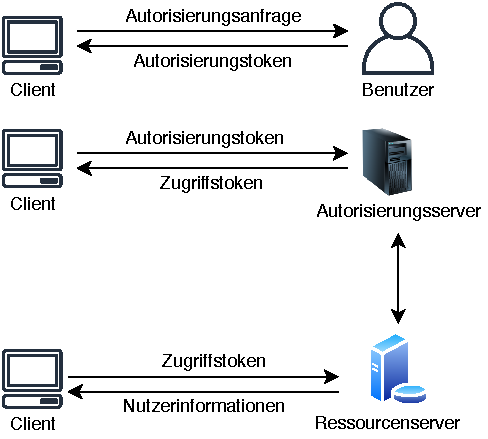
\includegraphics[width=.55\textwidth]{graphics/oauth2.pdf}
	\caption{oAuth2 verfahren}
	\label{fig:oauth2}
\end{figure}

%%% Local Variables:
%%% mode: latex
%%% TeX-master: "Tom - Thesis"
%%% End:

	\section{Anforderungsanalyse}
\label{sec: analyze}
Das Ziel dieser Thesis ist, ein standardisiertes Registrierungsverfahren zu erstellen, zuzüglich einer Authentifikation über \gls{oAuth2} oder ein Passwort. Hinzu kommt eine Möglichkeit, den Nutzer über den Server zu autorisieren und ihm nach spezifischen Benutzerrollen unterschiedlichen Inhalt zu präsentieren. Dabei soll es dem Nutzer nicht gestattet sein, durch Manipulation seines Clients mit verfälschten Daten, Zugriff auf für ihn nicht zugreiffbare Daten zu erhalten. Um das Ziel dieser Thesis zu erreichen, muss man sich vorerst mit Ruby und dem Webframework Rails auseinandersetzen. Zudem ist es vonnöten, sich intensiver mit Angular zu beschäftigen, da dieses bisher nur oberflächlich behandelt wurde.

\subsection{Derzeitiges Projekt}
\label{sec: current_project}
Zum derzeitigen Zeitpunkt ist Blattwerkzeug eine Lernplattform, in der jeder Nutzer jedes Projekt bearbeiten kann. Dafür wurde serverseitig ein Benutzername und Passwort, in beiden Fällen \enquote{user}, hinterlegt. Zusätzlich ist es möglich, das Adminpanel ohne weitere Autorisierungsabfrage zu betätigen.

\subsubsection{Client}
Der clientseitige Teil von Blattwerkzeug basiert auf Angular, Angular-Material und Bootstrap, hierbei sind Angular-Material und Bootstrap Gestaltungsframeworks. Bootstrap, welches hauptsächlich auf \gls{CSS} und \gls{HTML} basiert und Angular-Material, dass explizit Module für Angular bereitstellt.

\subsubsection{Server}
Der serverseitige Teil baut auf Ruby on Rails und bietet ein \gls{API} zur Kommunikation mit dem Server. Die Daten werden mittels unterschiedlicher Anfragemethoden abgefragt, übermittelt und vom Server verarbeitet.

\subsection{Anforderungen}
\label{sec: requirement}
Im Verlauf dieser Sektion werden die Anforderungen, die diese Thesis erfüllen soll, detailliert erläutert.

\subsubsection{Unterschiedliche Anmeldemöglichkeiten}
Ein Benutzer sollte die Möglichkeit haben sich mit mehreren Konten zu verknüpfen. Das bedeutet, einem Benutzer würde die Möglichkeit gegeben sein, sich mit Passwort und zum Beispiel Google anzumelden. 

\subsubsection{Anmeldung mittels \gls{oAuth2}}
Eine Authentifizierung mittels oAuth2 soll über Google und GitHub möglich sein. Die von Google oder GitHub zurückgelieferten Daten sollen in der Datenbank abgespeichert werden. Darüber hinaus müsste bei dem Vorhandensein spezifischer Daten, wie beispielsweise die einer E-Mail, eine automatische Zuweisung spezieller Datenbankfelder des Nutzers erfolgen.

\subsubsection{Anmeldung mittels Passwortes}
Für eine Anmeldung mittels Passwortes muss zuerst eine Möglichkeit verfügbar sein ein Konto zu erstellen. Bei der Erstellung eines Kontos sollten vier Felder geben sein. Das Erste für den Benutzernamen, das Zweite für die E-Mail, das Dritte und Vierte für das Passwort und die Passwort Bestätigung. Sobald der Benutzer seine Daten erfolgreich abgeschickt hat, würde das vom Client als Klartext verschickte Passwort auf dem Server verschlüsselt werden. Nachdem der Benutzer sein Konto erstellt hat, muss eine Bestätigungsmail an die angegebene E-Mail gesendet werden. Diese Bestätigungsmail sollte einen Hyperlink beinhalten mit dem das vom Nutzer erstellte Konto bestätigt werden kann. Empfängt diese E-Mail den Nutzer nicht, muss die Möglichkeit bestehen, eine erneute Bestätigungsmail zu versenden. Erst nachdem das Konto bestätigt wurde, soll es dem Nutzer gestattet sein, dieses Konto zu verwenden. Falls ein Nutzer sein Passwort vergessen hat, muss es zusätzlich eine Funktion zum Passwort wiederherstellen geben.

\subsubsection{Authentifizierung nach Anmeldung}
Um vom Server als angemeldeter Benutzer authentifiziert zu werden, müssen die Benutzerdaten in einem \gls{JWT} gespeichert werden. Dieser \gls{JWT} wird bei der Anmeldung eines Benutzers an den Client übermittelt. Ab dem Zeitpunkt wird dieser \gls{JWT} bei jeder Anfrage an den Server mit gesendet. Sobald eine Anfrage den Server erreicht, muss zwangsläufig der \gls{JWT} auf seine Gültigkeit geprüft werden. Hat dieser \gls{JWT} eine nicht gültige Signatur oder ist bereits abgelaufen, darf keine weitere Aktion auf dem Server erfolgen.

\subsubsection{Sicherheit und Login}
Die Einstellungen im Bereich Sicherheit und Login sollen einem Benutzer erlauben sein bereits erstelltes Konto mit weiteren Konten zu verknüpfen. Hierbei muss der Benutzer eingeloggt sein und einen bestimmten Provider auf seiner Einstellungsseite auswählen können. Nachdem sich der Benutzer bei dem ausgewählten Provider authentifiziert hat, sollte dieses Konto dem Nutzer hinzugefügt werden. Ebenso müssen die Benutzereinstellungen eine Verwaltung der verknüpften Konten beinhalten. Das bedeutet der Benutzer kann zu jeder Zeit entscheiden, welche dieser verknüpften Konten beständig bleiben oder welche gelöscht werden.

Hat sich ein Benutzer mittels Passwortes auf Blattwerkzeug registriert, muss es für diesen Nutzer eine Möglichkeit geben sein Passwort zu ändern, selbst wenn dieser bereits sein Konto zusätzlich mit Google oder GitHub verknüpft hat. Besteht für den Benutzer bereits ein vorhandenes Konto mit einem Passwort, sollte das neu zu verknüpfende Konto automatisch das Passwort des bereits Vorhandenen annehmen. Falls das zu verknüpfende Konto das erste mit einem Passwort sein sollte, muss dafür in den Benutzereinstellungen eine extra Passworteingabe dargestellt werden, in die das zu verwendende Passwort eingegeben wird.

Da es in Blattwerkzeug bei der Benutzernamensgebung zum jetzigen Stand keine einmaligen Benutzernamen gibt, muss es dem Benutzer in den Benutzereinstellungen zusätzlich möglich sein, seinen Benutzernamen zu ändern.

\subsubsection{Rollen und Autorisierung}
Die Rollen müssen sich in globale und Ressourcen spezifische Rollen unterteilen. Dabei sind Globale-Rollen wie in Sektion ~\ref{sec: rolify} beschrieben, keiner spezifischen Ressource zugewiesen. Zwei Beispiele globaler Rollen wären \enquote{user} und \enquote{admin} oder \enquote{guest}, \enquote{user} und \enquote{admin}. Ressourcen spezifische Rollen beziehen sich zum Beispiel auf ein Projekt. Bei der Erstellung eines Projektes muss ein Benutzer eine Rolle oder eine Datenbank-Beziehung zu dem jeweiligen Projekt erhalten. Mit dieser Rolle ist es dann dem Benutzer möglich, sein Projekt zu bearbeiten oder zu löschen. Zusätzlich muss die Möglichkeit gegeben sein, einem anderen Benutzer eine Rolle zuzuweisen mit der das Bearbeiten eines von ihm nicht erstellten Projektes ermöglicht wird. Administratoren mit der \enquote{admin} Rolle sollten jedoch Zugriff auf jedes Projekt haben.

\todo[inline]{Auflistung von nötigen Rollen und Rechten}

Für eine Autorisierung mittels Rollen müssen bestimmte Regeln für die jeweiligen Controller Funktionen festgelegt werden. Diese Regeln werden mittels Pundit erstellt werden. Innerhalb dieser Regeln sollte die Überprüfung der Rollen des angemeldeten Nutzers stattfinden.


\subsubsection{Bedienelemente und Routen}
Die Bedienelemente, die ein Benutzer zu sehen hat, müssen jeweils von den Rollen abhängen. Dazu ist es vonnöten, bei jedem Bedienelement den Server nach der Berechtigung zu fragen oder jedoch Clientseitig Pundit nachzubauen. Besucht ein Benutzer eine Route mit nicht ausreichender Berechtigung, wird ihm der Zugriff verwehrt. Die Bedienelemente sollten benuzterfreundlich sein, da es sich bei Blattwerkzeug, wie in Sektion \ref{sec:blattwerkzeug} beschrieben, um ein Werkzeug zum Lernen bestimmter Bereiche der Informatik handelt.

\todo[inline]{Code-Beispiel für Verwendung als Angular-Komponente (Template)}

	\section{Implementierung}
\label{sec: implementation}
In dieser Sektion wird sich ausgiebig mit der Implementierung der zuvor festgelegten Anforderungen auseinandergesetzt.

\subsection{Server}
\label{sec: server}
Da zu diesem Zeitpunkt bereits Librarys zur Authentifizierung existieren, wurde sich zuerst mit der Library Devise auseinandergesetzt.

\subsubsection{Devise}
\label{sec: devise}
Devise ist eine Ruby on Rails Library mit der sich eine flexible Authentifizierung ermöglichen lässt. Es bietet ein vorgefertigtes Datenbankschema für registrierte Benutzer, einen leichten Umgang mit OmniAuth und Funktionen wie beispielsweise das Senden einer E-Mail bei Registrierung. Im Datenbankschema enthalten ist ein Log-System mit dem beispielweise der Zeitpunkt der letzten Anmeldung eines Benutzers festgehalten werden kann. \todo{Warum nicht genommen? Was für Probleme traten auf?}


\subsubsection{Omniauth}
\label{sec:omniauth}
Omniauth ist eine quelloffene Library für Ruby on Rails und ermöglicht einem, eine Anmeldung mittels unterschiedlicher Anbieter über \gls{oAuth2}. Bei der Anmeldung mittels oAuth2 werden bereits viele Funktionen von Omniauth selber übernommen. Sobald der Nutzer sich bei dem jeweiligen Anbieter angemeldet hat, wird die Antwort des jeweiligen Anbieters automatisch über die von Omniauth festgelegte Route verarbeitet. Jedoch muss vorher das spezifische Gem des Anbieters für Omniauth installiert werden. Hierbei stellt jedes Gem eine eigene Strategie für Omniauth bereit. Eine Strategie stellt die Möglichkeit bereit sich mit einem speziellen Provider zu authentifizieren.

Omniauth selber verfügt nur über die Developer Strategie, diese ermöglicht eine Anmeldung ohne spezifische Überprüfung der angegebenen Daten. Das hat zur Folge, dass diese Art von Anmeldung auf keinen Fall im Produktiv System vorhanden sein darf.

Den Vorteil den Omniauth bietet ist die Kapselung zwischen den spezifischen Providern und der Hauptfunktionalität von Omniauth. Dies hat zur Folge, dass der Server nur explizit mit den installierten Providern kommunizieren kann. Außerdem bietet Omniauth eine lange Liste an zu installierenden Providern.

Beispiele an zu installierenden Providern: 
\begin{enumerate} 
	\item GitHub\footnote{https://github.com/omniauth/omniauth-github}
	\item GitLab\footnote{https://github.com/linchus/omniauth-gitlab}
	\item Goodreads\footnote{https://github.com/sandboxws/omniauth-goodreads}
	\item Google\footnote{https://github.com/Yesware/omniauth-google}
\end{enumerate}

\subsubsection{Pundit}
\label{sec: pundit}
Pundit ist eine Ruby on Rails Library die ein Designpattern zur Autorisierung bietet. Bei diesem Pattern wird zu einem jeweiligen Controller eine Policy angelegt. Eine Policy ist hierbei nur eine Klasse. Dabei setzt sich der Name der Policy, aus dem Namen des Models und dem Schlüsselwort Policy als Suffix zusammen. Dem Konstruktor der Policy wird beispielsweise ein Nutzer und das jeweilige Objekt übergeben, welches auf den Zugriff geprüft werden soll. Innerhalb der Policy werden die jeweiligen Controllerfunktionsköpfe in denen eine Autorisierung stattfinden soll mit einem \enquote{?} als Suffix ergänzt und definiert. Diese Funktionen müssen zwingend einen Boolean als Rückgabewert haben um eine gültige Auswirkung als Policy zu haben. Sobald die aufgerufene Funktion der Policy fehlschlägt wird eine Exception geworfen. Diese Exception kann an jeweiliger Position beispielsweise im Controller abgefangen und verarbeitet werden.

Da es sich bei Policies um Klassen handelt, können diese auch instanziiert und jeweilige Funktionen dynamisch abgerufen werden. Dies hat zur Folge, dass explizit nach einer bestimmten Policy-Funktion gefragt werden kann, selbst wenn der Funktionsname nicht dem der aufgerufenen Policy-Funktion entspricht.

\subsubsection{Rolify}
\label{sec: rolify}
Rolify ist eine Ruby on Rails Library zur Verwaltung von Rollen. Hierbei liefert Rolify bereits zwei Datenbanktabellen im Design der polymorphen Assoziation (Abbildung \ref{fig:server-polymorph-association}). Bei einer Eins-zu-viele-Assoziation hat beispielsweise ein Nutzer verschiedene Rollen, diese Rollen beinhalten verschiedene Fremdschlüssel aus verschiedenen Tabellen. Dabei ergibt sich das Problem, dass nicht mehr sicher gestellt werden kann aus welcher Tabelle der Fremdschlüssel stammt. Um dieses Problem zu lösen gibt es drei bewährte Methoden. In dieser Thesis gehen wir jedoch nur auf die von Rolify mitgelieferte Methode ein.

Bei dieser Methode handelt es sich um eine Kindtabelle \enquote{roles} und einer Elterntabelle \enquote{users\_roles}. Dabei stehen in der Roles-Tabelle die jeweiligen Informationen der Rolle und auf welche Ressource diese Rolle sich bezieht. Rolify unterscheidet hierbei zwischen globalen und Ressourcen spezifische Rollen. Eine globale Rolle beinhaltet keine Informationen einer Ressource und kann somit als beispielsweise allgemeine \enquote{user} Rolle dienen.

\begin{figure}[h]
	\centering
	\includegraphics[width=.6\textwidth]{graphics/rolify.pdf}
	\caption{Rolifys Datenbanktabellen mit Beziehung zur users Tabelle}
	\label{fig:server-polymorph-association}
\end{figure}

Die \enquote{users\_roles} beinhaltet wiederum die jeweilige \enquote{user\_id} und die zu dem Nutzer dazugehörigen Primärschlüssel einer Rolle. Dabei können verschiedene Nutzer dieselbe Rolle und ein Nutzer verschiedene Rollen haben.

Außerdem liefert Rolify bereits vordefinierte Funktionen mit denen es möglich ist, jeweilige Rollen eines Nutzers abzufragen, hinzuzufügen oder zu entfernen.



\subsubsection{Anmeldung eines Benutzers}
\label{sec: sign-in-imp}
Die Anmeldung mittels oAuth2 oder Passwort wurde mit Omniauth ermöglicht. Hierbei wurde zuerst Omniauth selber dem derzeitigen Projekt hinzugefügt und darauffolgend die Gems zur Authentifizierung mittels Google, GitHub und Passwort. Um die einzelnen Provider nutzen zu können müssen diese in einem initializer (Listing \ref{lst:added_providers}) deklariert werden. Ein initializer wird nach dem Rails Framework und den dazugehörigen Gems geladen. Bei der Deklarierung der Provider ist zu beachten, dass Provider wie Google oder GitHub eine jeweilige ID und einen Secret-Key als Parameter benötigen. Diese werden jeweils auf den offiziellen Seiten der Provider erstellt. Dabei musste darauf geachtet werden, dass diese ID und dieser Secret-key über eine Umgebungsvariable mit in das Projekt eingebunden wird. Umgebungsvariablen werden in dem Fall in der Kommandozeile vor das Kommando zum starten des Projektes gesetzt. Nach dem das Kommando zum starten des Servers ausgeführt wurde, kann auf die Werte der zuvor festgelegten Umgebungsvariablen zugegriffen werden. Die Verwendung von Umgebungsvariablen ist besonders bei Blattwerkzeug vonnöten, da es sich um ein quelloffenes Projekt handelt und jeder den bereits produzierten Code einsehen kann. Da es sich bei Secret-Keys um Passwörter handelt, sind diese nicht im Repository angegeben.  

\lstinputlisting[language=Ruby, style=CodeView, basicstyle=\scriptsize, caption=Zu Omniauth hinzugefügte Provider, captionpos=b, label={lst:added_providers}]{snippets/omniauth-initializer.rb}


Bei der Erstellung des User und des Identity Models wurde zuerst diskutiert welche Attribute die jeweiligen Models haben sollen. Hierbei steht das Identity Model für alle hinzugefügten Authentifikations-Möglichkeiten eines Benutzers. Dabei wurde darauf geachtet, welche Attribute später dem Client zur Verfügung gestellt werden sollten und welche für spätere Controller Funktionen benötigt werden.

\subsubsection*{Attribute der identities Tabelle}
Die nachfolgenden Beschreibungen der Attribute beziehen sich auf die identities Tabelle, welche in Abbildung \ref{fig:server-users-identities} dargestellt wird.
\begin{description}
	\item[uid]\hfill\\
	Die uid ist ein String der zur eindeutigen Identifikation des Kontos eines Providers dient. Dabei kann die uid beispielsweise eine Zahl oder eine E-Mail sein. Mit der uid wird festgestellt ob ein bestimmtes Konto bereits mit einem Benutzer verknüpft ist.
	\item[provider]\hfill\\
	Das provider Attribut wird mit dem jeweiligen Provider-Namen beschrieben. Dabei sind die Namen wie in Listing \ref{lst:added_providers} definiert. Da die Namen jedoch von den installierten Gems definiert werden, ist eine Änderung dieser Namen nicht ohne weiteres Möglich.
	\item[provider\_data]\hfill\\
	Das provider\_data Attribut wird mit jeglichen Daten beschrieben, die ein Provider über den authentifizierten Benutzer zurückliefert. (Listing \ref{lst:server-github-oauth-data} \& \ref{lst:server-google-oauth-data})
	
	\begin{minipage}{.42\textwidth}
		\lstinputlisting[language=JSON, style=CodeView, basicstyle=\scriptsize, caption=GitHubs oAuth Daten, captionpos=b, label={lst:server-github-oauth-data}]{snippets/github-provider-data.json}
	\end{minipage}\hfill
	\begin{minipage}{.42\textwidth}
		\lstinputlisting[language=JSON, style=CodeView, basicstyle=\scriptsize, caption=Googles oAuth Daten, captionpos=b, label={lst:server-google-oauth-data}]{snippets/google-provider-data.json}
	\end{minipage}
	
	\item[own\_data]\hfill\\
	Das own\_data Attribut wird mit den Daten beschrieben die Blattwerkzeug für den Benutzer vorgesehen hat. Dies kann beispielsweise der Token zur Aktivierung einer E-Mail sein.
	\item[type]\hfill\\
	Das type Attribut wird, sobald es der Tabelle hinzugefügt wurde, von Rails automatisch interpretiert. Hierbei handelt es sich um \gls{STI}. \gls{STI} ist eine Möglichkeit Objekt-Orientierung in einer Relationellen Datenbank zu emulieren. Dabei ist die Tabelle identities und dessen Model (Identity) die Basisklasse und die in type festgelegten Klassen, die Abgeleiteten. Das type Attribut ermöglicht einen sofortigen Zugriff auf die Klasse des Providers einer ausgewählten Identity.
\end{description}

\begin{figure}[h]
	\centering
	\includegraphics[width=0.7\textwidth]{graphics/users-identities.pdf}
	\caption{Darstellung der users und identities Tabelle inklusive Beziehung.}
	\label{fig:server-users-identities}
\end{figure}

\subsubsection*{Attribute der users Tabelle}
Die nachfolgenden Beschreibungen der Attribute beziehen sich auf die users Tabelle, welche in Abbildung \ref{fig:server-users-identities} dargestellt wird.
\begin{description}
	\item[display\_name]\hfill\\
	Das display\_name Attribut steht für den Anzeigenamen des Benutzers. Dieser ist jedoch nicht einzigartig und lässt sich beliebig oft verändern. Das hat zur Folge, dass mehrere Benutzer denselben Anzeigenamen haben können.
	\item[email]\hfill\\
	Das email Attribut steht für die primäre E-Mail eines Benutzers. Die primäre E-Mail wird verwendet sobald eine E-Mail von Blattwerkzeug an den Benutzer gesendet werden soll. Dies ist wichtig, da jedes verknüpfte Konto eine unterschiedliche E-Mail besitzen darf. Die primäre E-Mail wird bei Erstellung eines Benutzers gesetzt, außer ein Benutzer authentifiziert sich über einen Provider dessen Rückgabe keine E-Mail enthält.
\end{description}

\subsubsection*{Anmeldemöglichkeiten}
Die geforderten Anmeldemöglichkeiten und deren Implementierung werden in diesem Abschnitt erläutert. 
\begin{description}
	\item[Anmeldung mittels \gls{oAuth2}]\hfill\\
	Bei einer Anmeldung mittels \gls{oAuth2} wurde bei dem Provider über den sich authentifiziert wird, eine Redirect Url hinterlegt. Auf diese wird der jeweilige Benutzer nach Authentifikation zurückgeleitet. Die Route zu der Redirect Url zeigt auf die Funktion mit dem Namen \enquote{Callback} im \enquote{AuthController}. Die Callback Funktion prüft auf das vorhanden sein der vom Provider zurückgelieferten Daten. Sollte bisher keine Identität mit den Daten des Providers erstellt worden sein wird eine neue Identität angelegt. Sollte ein angemeldeter Benutzer diese Funktion ausführen wird ihm eine neue Identität zu seinem Benutzer hinzugefügt. Sollte es sich um keinen angemeldeten Benutzer handeln, wird zusätzlich ein neuer Benutzer erstellt. Da jeder Provider unterschiedliche Daten zurückliefert wird beim anlegen einer neuen Identität zwischen den einzelnen Providern unterschieden. Jeder Provider besitzt eine Abgeleiteteklasse der Basisklasse Identity und greift innerhalb seiner Klasse auf die für ihn relevanten Daten zu. Sollte eine Identität mit den zuürckgelieferten Daten bereits existieren, wird ohne Erstellung einer Identität fortgefahren. Mit der erstellten oder existierenden Identität werden die Benutzerinformationen in die Payload eines \gls{JWT} geschrieben. Bei den Benutzerinformationen handelt es sich um die id, den display\_name und die Rollen eines Benutzers. Die Funktionen zu Erstellung eines \gls{JWT} wurden hierbei in einen Helper ausgelagert und die Gültigkeitsdauer des erstellten \gls{JWT} beläuft sich auf eine Stunde.

	\begin{figure}[h]
		\centering
		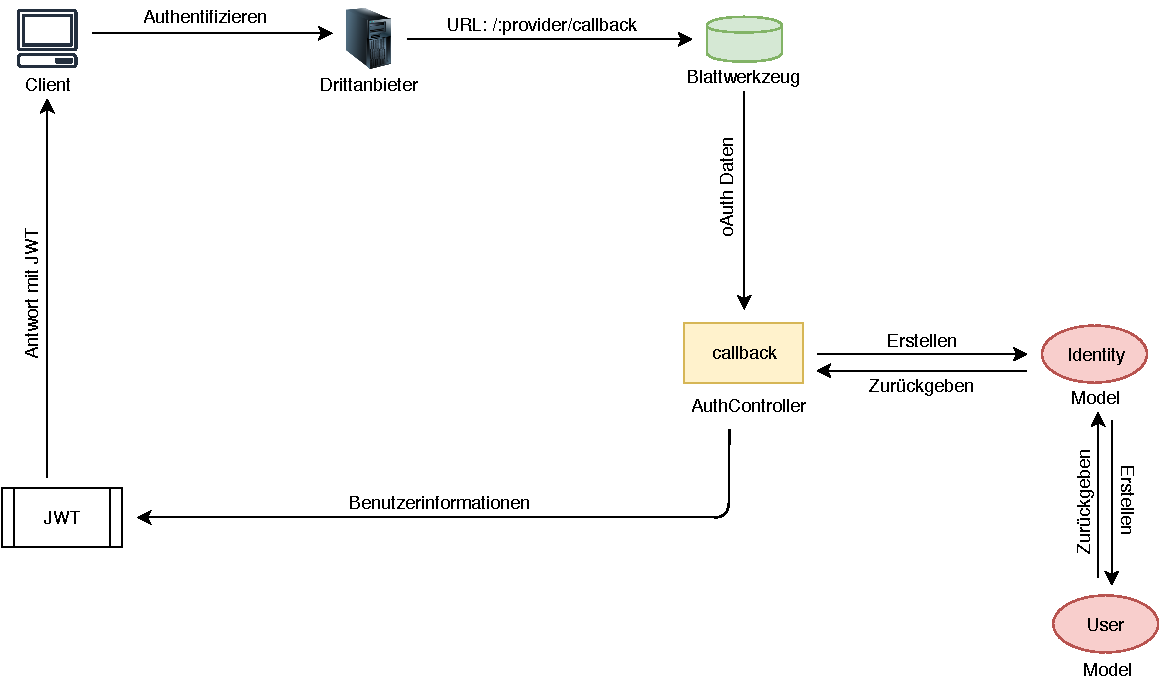
\includegraphics[width=0.6\textwidth]{graphics/sign-in-oauth2.pdf}
		\caption{Ablauf einer Anmeldung mittels \gls{oAuth2}}
		\label{fig:server-sign-in-oauth}
	\end{figure}

	\item[Anmeldung mittels Passwort]\hfill\\
	\todo[inline]{Visualisierung als Automat (Zustände / Übergänge) zur Veranschaulichung des Prozesses vermutlich hilfreich}
	\todo[inline]{Allgemein: Mehr Struktur, in diesem Punkt verstecken sich zuviele eigenständige Funktionen}
	Die Anmeldung mittels Passwort wurde mittels Omniauth Identity\footnote{\url{https://github.com/omniauth/omniauth-identity}} ermöglicht. Omniauth Identity ist ebenfalls eine Strategie mit der die Möglichkeit gegeben ist, sich über ein Passwort bei Blattwerkzeug anzumelden. Ebenso wie die Developer Strategie, bietet auch diese Strategie die Möglichkeit ein vorgefertigtes Formular für Anmeldung und Registrierung zu erstellen. Jedoch ist es bei dieser Strategie optional und eine ausschließliche Kommunikation über ein API ist möglich.

	Bei dem Nutzen dieser Strategie fiel auf, dass die Daten übermittelt wurden sie jedoch nicht richtig verarbeitet werden konnten (Listing \ref{lst:register_omniauth_identity}). Das hatte zur Folge, dass mit der Erstellung eines Models, welches mit als Parameter im iniziliazer angegeben werden kann, nicht ordnungsgemäß fortgefahren werden konnte. Um fortzufahren wäre es möglich eine eigene Strategie für Omniauth zu entwickeln oder auf die von Omniauth Identity mitgelieferten Optionen zurück zugreiffen.
	
	\begin{minipage}{\textwidth}
		\lstinputlisting[language=Ruby, style=CodeView, caption=Aufgerufene Funktion bei POST Request (Omniauth Identity), captionpos=b, label={lst:register_omniauth_identity}]{snippets/omniauth-identity-registration.rb}
	\end{minipage}

	Omniauth Identity bietet die Möglichkeit bei Registrierung auf eine Funktion zu verweisen. Diese Funktion muss ebenfalls im iniziliazer\todo{typo} angegeben werden. (Listing \ref{lst:added_providers}). Sollte bei der Erstellung des Models ein Fehler auftreten (Listing \ref{lst:register_omniauth_identity}), wird die Funktion im zuvor festgelegten iniziliazer aufgerufen. Letztendlich wurde sich in der Thesis für diese Methode entschieden. Hierbei wurden jegliche Funktionen innerhalb des AuthControllers und außerhalb der Strategie genutzt.

	Bevor eine Anmeldung mittels Passwort stattfinden kann, wurde eine Registrierungs-Möglichkeit hinzugefügt. Die \enquote{register} Funktion arbeitet ähnlich wie die callback Funktion\todo{welche}. Der Unterschied besteht darin, dass die register Funktion einen simulierten Hash in der Struktur Omniauths erhält und mit diesem versucht eine neue Identität zu erstellen. Beim erstellen einer neuen Password-Identität wird ein Verifizierungs-Token generiert. Dieser Verifizierungs-Token ist eine \gls{UUID} und wird zur Verzifizierung der Identität genutzt. Nachdem eine Identität erstellt wurde, sendet der Server mithilfe der Basisklasse ActionMailer eine Bestätigungsmail. Diese Bestätigungsmail verhindert das Registrieren von willkürlichen E-Mail Adressen. Außerdem wird  mit der Bestätigungsmail eine E-Mail Adresse auf ihre existens geprüft. Die Bestätigungsmail besteht aus einem Hyperlink zu einer \gls{URL} Blattwerkzeugs in der, der Verifizierungs-Token enthalten ist. Sobald dieser \gls{URL} besucht wird, wird die Indentität als bestätigt gekennzeichnet. Dies erfolgt durch das Setzen des confirmed Feldes im JSON Blob Attribut own\_data.

	Da es vorkommen kann, dass eine Verifizierungsmail nicht an der angegebene E-Mail ankommt, wurde hierfür eine Funktion im IdentitiesController geschrieben. Diese Funktion prüft die übermittelte E-Mail auf ihre existens in der Blattwerkzeug-Datenbank und ob diese bereits verifiziert wurde. Sollte diese E-Mail nicht verifiziert sein wird eine neue Verifizierungsmail versendet. Gleichzeitig wird jedoch auch eine Wartezeit von zwei Minuten im own\_data Attribut festgelegt. Die Wartezeit zum versenden einer neuen Verifizierungsmail soll verhindern, dass eine E-Mail Adresse mit Verifizierungsmails überhäuft werden kann.

	Sollte eine Identität mit einem Passwort bereits vorhanden sein, kann sich mit seiner E-Mail und seinem Passwort angemeldet werden. Bei der Anmeldung wird das Passwort zur angegebenen E-Mail überprüft. Zusätzlich wird geprüft ob die E-Mail verifiziert wurde. Sollten diese Sicherheitsabfragen erfolgreich durchlaufen sein wird wie bei der Anmeldung mittels \gls{oAuth2} ein \gls{JWT} ausgestellt in dem die Benutzerinformationen gespeichert werden.

	Da im Laufe der Zeit die Möglichkeit besteht, dass Benutzer ihr Passwort vergessen haben, wurde hierfür eine Funktion im IdentitiesController erstellt. Damit ein Passwort zurück gesetzt werden kann muss die übermittelte E-Mail Adresse als Passwort Identität vorhanden sein. Sollte diese Identität vorhanden sein, wird ein password\_reset\_token erstellt. Dieser password\_reset\_token ist eine \gls{UUID} und wird im own\_data JSON Blob Attribut gespeichert. Ebenfalls zum own\_data Attribut hinzugefügt wird ein Feld password\_reset\_token\_exp. Dessen Wert beläuft sich auf die aktuelle Uhrzeit plus dreißig Minuten. Nachdem die festgelegte Uhrzeit des password\_reset\_token\_exp Feldes überschritten wurde, kann der Zurücksetzungs-Token nicht mehr verwendet werden. Damit das Passwort trozdessen zurückgesetzt werden kann, muss ein neuer Zurücksetzungs-Token angefordert werden. Die Ablaufzeit eines Zurücksetzungs-Tokens hat den Vorteil, dass sollte beispielsweise ein Angreiffer Zugriff auf den Browserverlauf haben, dieser nicht die Möglichkeit erhält das Passwort dieses Benutzers zu verändern. Die E-Mail die beim Kennwort zurücksetzen versendet wird, wird an die primäre E-Mail verschickt und enhält einen Hyperlink zum wiederherstellen des Passwortes. Der Hyperlink beinhaltet den password\_reset\_token und nachdem ein neues Passwort ausgewählt wurde, wird von jeder Passwort-Identität des Benutzers das Passwort geändert.
\end{description}

\subsubsection{Autorisierung}
\label{sec:server-authorisation}
Sobald ein Benutzer angemeldet ist, wird bei jedem Request ein \gls{JWT} mit an den Server gesendet. Dieser wird Serverseitig auf seine Gültigkeit geprüft. Hierbei prüft der Server ob dieser \gls{JWT} seine Ablaufzeit nicht überschritten hat und ob der \gls{JWT} die Signatur des Servers beinhaltet. Diese Überprüfung authentifiziert einen Besucher als angemeldeten Benutzer und wird von der Library jwt\footnote{\url{https://github.com/jwt/ruby-jwt}} übernommen.

Damit zwischen den Benutzern unterschieden werden kann, wurden drei Globale-Rollen eingebaut.

\todo[inline]{Unklar: Was genau wurde extra \enquote{eingebaut}? Ich halte das eher für eine Konvention. Und zwischen Benitzern unterscheidet man anhand ihrer ID ;-) Ich weiß was gemeint ist, aber geh hier nochmal in dich und formulier sauber aus inwiefern diese (sinnvolle!) Konvention dir hilft.}

\begin{description}
	\item[guest]\hfill\\
	Die guest Rolle wird einem einzigen Benutzer zugewiesen. Dieser Benutzer beschreibt einen unangemeldeten Besucher. Jedem der Blattwerkzeug besucht und sich nicht anmeldet wird dieser Gast-Benutzer zugewiesen. Der Gast-Benutzer besitzt keine Möglichkeit Änderungen, die über Bedienelemente ermöglicht werden, zu speichern oder zu löschen.
	\item[user]\hfill\\
	Die user Rolle stellt einen angemeldeten Benutzer dar. Sollte bei einer Identitäts Erstellung festgestellt werden, dass der aktuelle Benutzer keine Globale-Rolle admin oder user besitzt, wird automatisch die user Rolle hinzugefügt. Mit der user Rolle wird das Erstellen, Speichern und Löschen von Projekten ermöglicht. Dies bezieht sich jedoch nur auf eigene Projekte.
	\item[admin]\hfill\\
	Die admin Rolle stellt einen administrierenden Benutzer dar. Jegliche Operationen die mit der user Rolle ausgeführt werden können, können ebenfalls mit der admin Rolle ausgeführt werden. Darüberhinaus kann ein Benutzer mit der admin Rolle, jegliche Projekte bearbeiten und beschränkt sich nicht auf seine eigenen. Der Admin-Benutzer besitzt zusätzliche Funktionen mit denen er beispielsweise eine Neuigkeit, die Clientseitig auf der Startseite angezeigt wird, erstellen kann.
\end{description}

Um den Zugriff auf das Verwalten eines Projektes oder einer News zu beschränken, wurde jeweils eine Policy (Listing \ref{lst:project_policy}) angelegt. Bei der Erstellung einer Policy fiel auf, dass es sinnvoller ist den Ersteller einer News oder eines Projektes in der jeweiligen Tabelle mit zu hinterlegen. Dafür wurde ein neues Attribut owner der projects und news Tabelle hinzugefügt. Dieses owner Attribut ist ein Fremdschlüssel und bezieht sicht auf die users Tabelle. Die Beziehung die folgedessen enstand ist eine 1:n. Das beudetet ein Benutzer kann beispielsweise verschiedene Projekte besitzen, jedoch ein Projekt nur einen Benutzer haben. Den Vorteil den das hinzufügen des owner Attributes hat, ist der direkte Zugriff auf die erstellten Projekte eines Benutzers. Außerdem kann zwischen einem Ersteller eines Projektes und einem Benutzer der eine Rolle zum bearbeiten eines Projektes erhalten hat, unterschieden werden kann.

\begin{minipage}{\textwidth}
	\lstinputlisting[language=Ruby, style=CodeView, caption=Policy zur Autorisierung eines Zugriffs auf ein Projekt, captionpos=b, label={lst:project_policy}]{snippets/project_policy.rb}
\end{minipage}

Da Blattwerkzeug bereits eine Passwortabfrage eingebaut hatte (Listing \ref{lst:controller_function_before}) dessen Anmeldedaten sich auf user und user beschränkten, mussten diese durch die von Pundit mitgelieferte authorize (Listing \ref{lst:controller_function_after}) Methode ersetzt werden.

\begin{minipage}{\linewidth}
	\lstinputlisting[language=Ruby, caption=Controller-Funktion ohne Integrierung Pundits, style=CodeView, captionpos=b, label={lst:controller_function_before}]{snippets/controller_authorisation_before.rb}
\end{minipage}

\begin{minipage}{\linewidth}
	\lstinputlisting[language=Ruby, caption=Controller-Funktion mit Integrierung Pundits, style=CodeView, captionpos=b, label={lst:controller_function_after}]{snippets/controller_authorisation_after.rb}
\end{minipage}

\subsubsection{may\_perform}
Sobald sich mit den Rollen beschäftigt wurde, stellte sich die Frage wie die Bedienelemente in Abhängigkeit von den Rollen Clientseitig angezeigt werden sollten. Hierbei gab es die Möglichkeit ein eigenes Pundit (Sektion \ref{sec: pundit}) ähnliches Mustur zu implementieren oder den Server bei jedem Bedienelement zu fragen, ob der aktuelle Benutzer Zugriff auf das Bedienelement hat. In der Thesis wurde sich für den zweiten Weg entschieden, da bei einer zusätzlichen Clientseitigen Überprüfung, Client und Server gepflegt werden müssten. Sollte es vorkommen, dass die Pflege des Serverseitigen-Teils vergessen wurde, stellt dieses ein Sicherheitsrisiko dar. Clientseitige Anwendungen werden auf dem Entgerät eines Benutzers ausgeführt. Folgedessen besteht die Möglichkeit die Anwendung zu manipulieren.

Die Serverseitige Überprüfung der Bedienelemente wurde mittels der may\_perform Funktion realisiert. Diese erhält vom Client eine Liste an Daten in der jedes Element ein Bedienelement darstellt. In der may\_perform Funktion wird jedes Element der Liste durchlaufen und auf das Zugriffsrecht des aktuellen Benutzers geprüft. Dies geschieht in dem aus den übermittelten Daten eine Instanz einer Policy erstellt wird die zu der jeweiligen Ressource, beispielsweise der Projekte (Listing \ref{lst:project_policy}) gehört. Hierbei wird die Funktion die auf ihren Zugriff geprüft werden soll, ebenfalls vom Client mit an den Server gesendet. Diese wird schlussendlich auf der erstellten Instanz ausgeführt. Das Ergebnis der Aufgerufenen Policy Funktion wird in einem Array gespeichert und sobald die Liste durchlaufen wurde an den Client übermittelt. Die Nutzung des Arrays und der übermittelten Liste wird in der Client Sektion \ref{sec: client} erläutert.

\subsubsection{Sicherheit und Login}
\label{sec:server-account-settings}
Da ein Benutzer die Möglichkeit haben soll seinen Account zu verwalten und Änderung an diesem vorzunehmen, wurden fünf Einstellungsmöglichkeiten implementiert. Damit ein Benutzer Einstellungen an seinem Account vornehem kann, muss dieser sich vorerst anmelden.

\begin{description}
	\item[Konto verknüpfen]\hfill\\
	Die callback Funktion im Authcontroller enthält eine Abfrage zur Überprüfung eines angemeldeten Benutzers. Bei einem angemeldeten Benutzer wird die zuerstellende Identität dem angemeldeten Account hinzugefügt. Dies wird mittels eines Fremdschlüssels, der auf die id eines Benutzers referenziert, realisiert.
	\item[Konto löschen]\hfill\\
	Damit eine Identität gelöscht werden kann müssen zuerst einige Sicherheitsabfragen durchlaufen werden. Die E-Mail der zu löschenden Identität darf nicht als derzeitige primäre E-Mail fungieren. Folgedessen kann beim einem Fremdzugriff auf den Account, keine Übernahme des Benutzers erfolgen. Ebenfalls muss eine weitere bestätigte Identität vorhanden sein. Demnach ist es nicht möglich jegliche Authentifizierungs Möglichkeiten eines Benutzers zu entfernen. Um zu verhindern, dass mit verfälschten Daten fremde Identitäten gelöscht werden, muss die zu löschende Identität zwangsläufig dem angemeldeten Benutzer angehören.
	\item[Primäre E-Mail wechseln]\hfill\\
	Ein Benutzer hat die Möglichkeit die primäre E-Mail zu ändern. Hierbei wurde darauf geachtet, dass die Änderung einer primären E-Mail ebenfalls bestätigt werden muss. Das Bestätigen einer Änderung der primären E-Mail schützt vor Benutzer übernahmen innerhalb Blattwerkzeugs. Bei einer Änderung der primären E-Mail wird eine Bestätigungsmail vom Server gesendet, allerdings wird vorher überprüft ob die neue E-Mail in einem der verknüpften Identitäten vorhanden ist. Folglich ist es nicht Möglich mit manipulierten Daten, auf eine nicht verknüpfte und nicht bestätigte E-Mail zu wechseln. Die Bestätigungsmail enthält einen Hyperlink mit einem zuvor erstellten change\_primary\_email\_token. Damit die neue primäre E-Mail nicht als beispielsweise URL-Parameter mit an die \gls{URL} gehängt werden muss, wurde der change\_primary\_email\_token in der Identität der neuen primären E-Mail gespeichert. Demnach kann mittels Token direkt auf die wechselnde Identität zugegriffen werden. Für eine erfolgreiche Änderung der primären E-Mail, muss der an die \gls{URL} angehängte Token dem change\_primary\_email\_token entsprechen. Zusätzlich darf der angegebene Token seine Ablaufzeit nicht überschritten haben. Sollte die vom Benutzer ausgewählte E-Mail bereits als primäre E-Mail eines anderen Benutzers dienen, kann der Vorgang zur Änderung ebenfalls nicht erfolgreich abgeschlossen werden.
	\item[Passwort wechseln]\hfill\\
	Damit ein Passwort wechsel durchgeführt werden kann, muss eine Passwort Identität vorhanden sein. Um das Passwort der Passwort Identität zu verändern muss das derzeitige Passwort und eine neues Passwort, an den Server übermittelt werden. Der Server gleicht das übermittelte Passwort mit dem Passwort der verknüpften Identität ab. Sollten bereits mehrere Passwort Identitäten existieren, wird von jeder das Passwort geändert. Da bei einer Verknüpfung einer Passwort Identität, das Passwort einer bereits existierenden Passwort Identität übernommen wird, führt das ändern jeglicher Passwort Identitäten zu keinem ungewollten verhalten.
	\item[Benutzernamen wechseln]\hfill\\
	Da es in Blattwerkzeug keine eindeutigen Benutzernamen gibt, wurde eine Funktion zum wechseln des Benutzernamens hinzugefügt. Diese Funktion prüft lediglich auf das Valide sein eines Benutzers nach Änderung des Benutzernamens. Zur Überprüfung des Benutzernamens wurde ein Validator hinzugefügt, der den Benutzernamen mittels Regulären Ausdrucks auf seine Gültigkeit prüft. (Listing \ref{lst:validation_display_name}) Der Benutzername muss mit drei Buchstaben oder Zahlen beginnen und kann gefolgt werden von siebzehn Zeichen.

\end{description}

\lstinputlisting[language=Ruby, style=CodeView, caption=Validierung des Benutzernamens, captionpos=b, label={lst:validation_display_name},float,floatplacement=h]{snippets/email_validator.rb}

\todo[inline]{Die Regex-Regel ist so nicht sinnvoll. Webseiten beschränken Benutzernamen vor allem um Probleme mit leicht zu verwechselnden Zeichen zu vermeiden (Stichwort \enquote{Greek Question Mark Prank}) oder weil Namen wie \enquote{<script>alert(haha)</script>} gar nicht erst möglich sein sollen. Beschreibe beide Sachverhalte / Probleme (nicht unbedingt hier, das kann sogar bis zu den Anforderungen nach vorne) und präsentiere hier dann einen passenderen RegEx.}

\subsection{Client}
\label{sec: client}
Die Client Sektion beschreibt die Umsetzung der Anforderungen (clientseitig). 

\subsubsection{Nebular}
\label{sec: nebular}
Nebular ist eine Angular Library die bereits viele Bedienelemente im benutzerfreundlichen Design enthält. Zusätzlich stellt Nebular bereits Services und Helper Koponenten mit denen der Umgang mit \gls{oAuth2} oder \gls{JWT} erleichtert wird. Da Nebular jedoch eine so umfangreiche Libraby ist und wir im Fall dieser Thesis nur auf die Struktur und das Design der Bedienelemente zurückgegriffen hätten, wäre eine Vielzahl an zusätzlichen Eigenschaften Nebulas ungenutzt. Zusätzlich konzentriert sich Nebular bei Autorisierung stark auf den Clientseitigen Teil. Dies hat zur Folge, dass serverseitig und clientseitig Fehler abgefangen werden müssten. Aus diesen Gründen wurde sich gegen Nebular und für ein eigenes Design entschieden.

\subsubsection{Dialog zur Anmeldung/Registrierung}
\label{sec:client-dialog-authentication}
Zuerst wurde sich mit der Darstellung von Komponenten für die Anmeldung und die Registrierung auseinandergesetzt\todo{ugs}. Diese sollten einem neumodischen Stil entsprechen und leicht zu bedienen sein\todo{Dieser Satz beschreibt Anforderungen}. Hierbei bietet Angular Material eine Möglichkeit, sogenannte Dialog-Fenster zu erstellen. Um das Dialog-Fenster zu implementieren muss ein Modul namens \enquote{MatDialogModule} eingebunden werden. Angular Material bietet außerdem die Möglichkeit sogennante \enquote{tabs} zu verwenden. Diese Tabs ermöglichen den wechsel zwischen unterschiedlichem Inhalt mit zusätzlicher Animation und gleichbleibender Komponente. Aus diesen beiden Elementen von Angular Material wurde schluessendlich ein Popup-Fenster erstellt in dem der Wechsel zwischen Anmeldung (Abbildung~\ref{fig:dialog_sign_in}) und Registrierung (Abbildung~\ref{fig:dialog_sign_up}) ermöglicht wird.

\begin{figure}
	\centering
	\begin{subfigure}{.5\textwidth}
		\includegraphics[width=.95\linewidth]{graphics/dialog-sign-in.png}
		\caption{Darstellung eines Dialogs zur Anmeldung}
		\label{fig:dialog_sign_in}
	\end{subfigure}%
	\begin{subfigure}{.5\textwidth}
		\includegraphics[width=.95\linewidth]{graphics/dialog-sign-up.png}
		\caption{Darstellung eines Dialogs zur Registrierung}
		\label{fig:dialog_sign_up}
	\end{subfigure}
	\caption{Dialog zur Anmeldung/Registrierung}
	\label{fig:auth-dialog}
\end{figure}

\begin{description}
	\item[Kommunikation mit dem Server]\hfill\\
	Die Kommunikation mit dem Server findet mittels \gls{HTTP}-Anfragen statt. Um eine \gls{HTTP}-Anfrage zu ermöglichen, wird das \gls{HTTP}-Modul von Angular verwedent.

	Während der Arbeit mit Blattwerkzeug, wird ein Entwickler zwangsläufig mit dem Caching-System konfrontiert. Dieses speichert den zuletzt erhaltenen Wert einer \gls{HTTP}-Anfrage. Sollte auf das Observable, welches für die \gls{HTTP}-Anfrage zuständig ist, erneut zugegriffen werden, wird der gespeicherte Wert zurückgegeben. Ein gespeicherter Wert wird erst verändert, sobald explizit eine neue Anfrage an den Server gestellt wird.
	
	Für die Kommunikation mit dem Server wurde mit dem bereitgestellten Caching-System gearbeitet. Damit die zu übermittelnden Daten einer Datenstruktur zugeordnet werden können, wurden Interfaces erstellt. Das Verwenden eines Interfaces als Datenstruktur erleichtert die Identifikation der Zugehörigkeiten der zu übermittelnden Daten. 

	\item[Provider-Buttons]\hfill\\
	Damit zwischen Produktiv-, Entwicklungs-, und Testumgebung unterschieden werden kann, erhalten die Provider Buttons ihre Informationen mittels get Anfragemethode vom Server. Dies bietet den Vorteil, dass Serverseitig definiert werden kann, welche Provider dem Benutzer zur Authentifizierung bereit gestellt werden sollen.

	Die Darstellung der Provider-Buttons wird in zwei Komponenten unterteilt. Die provider-button Komponente dient der Darstellung des einzelnen Buttons. Diese enthält jegliche Informationen über den Provider und die Darstellung des Buttons. Die provider-all-buttons Komponente zeigt restlos jeden derzeitig verfügbaren Provider an. Innerhalb der provider-all-buttons Komponente wird auf die provider-button Komponenten zurückgegriffen.
	\item[Validate-Input]\hfill\\
	Der Auth-Dialog beinhaltet verschiedene Input-Felder. Um eine Rückmeldung bei Fehleingabe in einem der Input-Felder zu erhalten, muss ein Input-Feld validiert werden. Hierbei sind verschiedene Möglichkeiten gegeben.

	Die Validierung eines Input-Feldes ist ein fester bestandteil\todo{typo} von \gls{HTML}5. Für eine Validierung mittels \gls{HTML}5 Validator, muss der Validator als Attribut dem Input-Feld hinzugefügt werden. 
	
	Die Angular Validierung bietet bereits vordefinierte Klassenmethoden zur Validierung von Input-Feldern. Die vordefinierten Klassenmethoden gleichen, von der Funktionsweise, den HTML Validatoren. Ein Vorteil den Angular hierbei bietet, ist das Erstellen eigener komplexer Validatoren. Ein weiterer Vorteil, ist das Auslagern der Validatoren aus dem Template. Folglich kann beispielsweise ein Service zur Validierung von Input-Feldern dienen und somit anwendungsübergreifend die Validierung geändert werden.

	Für die Entscheidung zwischen \gls{HTML}5 und Angular Validierung, musste abgewägt werden in welchem Umfang die Validierung benötigt wird. Die zu Nutzenden Input-Felder können jeweils mit den vordefinierten Validatoren, beider Validierungs-Möglichkeiten, validiert werden. Aus diesem Grund wurde sich für die \gls{HTML}5 Validierung entschieden, da diese über das Hinzufügen als Attribut eine deutlich komfortablere Lösung bietet.

	Bei der Implementierung der jeweiligen Validatoren innerhalb der Input-Felder wurde erhöhte Code-Redundanz festgestellt. Aus diesem Grund wurde für das Validieren der einzelnen Input-Felder eine validate-input Komponente erstellt. Die validate-input Komponente lädt dynamisch ein Input-Feld mittels ng-content in das Template. Der zu validierende Wert, wird mittels input-binding an die validate-input Komponente übermittelt (Listing \ref{lst:validate_input}). Zusätzlich kann mit input-binding das Design des Input-Feldes (Abbildung \ref{fig:validate_input}) erweitert werden. Sollte die Validierung des übermittelten Wertes fehlschlagen, wird undefined an die Eltern-Komponente zurückgeliefert. Dies hat den Vorteil, dass der Client von einem invaliden Wert ausgehen kann und der Server keine invaliden Werte, außer undefined, erhält. Allerdings verhindert diese Komponente nur bei falscher Eingabe das Übermitteln von falschen Daten. Aus diesem Grund ist diese Komponente kein Ersatz für die serverseitge Validierung.

	\begin{figure}
		\centering
		\includegraphics[scale=0.7]{graphics/validate-input-example.pdf}
		\caption{Standart und erweiterte Ausführung eines validate-input}
		\label{fig:validate_input}
	\end{figure}
	\todo[inline]{Standard! Und verpass den Icons mal die CSS-Klasse fa-fw, dann werden die identisch breit dargestellt.}


	\begin{minipage}{\linewidth}
			\lstinputlisting[language=JavaScript, style=CodeView, caption=Verwendung einer validate-input Komponente, captionpos=b, label={lst:validate_input}]{snippets/validate_input.ts}
	\end{minipage}

	\item[Inspiration]\hfill\\
\end{description}

\subsubsection{Speichern eines \gls{JWT}}
Bei dem erstellen eines \gls{JWT} muss abegewägt werden wo dieser Clientseitig gespeichert werden soll. Hierbei gibt es die Möglichkeit den \gls{JWT} im LocalStorage, sessionStorage oder als Cookie zu speichern.

Der LocalStorage und der sessionStorage sind ähnlich und bieten dieselben schwachstellen, weßhalb sich im weiteren Verlauf nur auf den LocalStorage bezogen wird. Bei der Speicherung eines \gls{JWT} im LocalStorage wird \gls{XSS} zur Schwachstelle. Bei \gls{XSS} handelt es sich um mit einer der bekanntesten Angriffsmethoden in der Webentwicklung. Hierbei wird beispielsweise ein Hyperlink manipuliert und mit \JS auf den localStorage zugegriffen. Sobald sich ein Angreifer den \gls{JWT} zukommen lassen hat, ist es für diesen möglich sich mit dem \gls{JWT} zu authentifizieren. Angular schützt seine Applikationen bereits vor \gls{XSS} in dem beispielsweise Eigenschaften und Attribute auf nicht vertrauenswürdige Werte überprüft werden.

Die Speicherung im Cookie bietet die Möglichkeit, mit dem httpOnly-Flag, den Zugriff mittels \JS zu verbieten. Zusätzlich kann der secure-Flag gesetzt werden, der die Übertragung des Cookies nur über eine sichere \gls{HTTPS} Verbindung zulässt. Jedoch hat die Speicherung eines Cookies ebenfalls eine große Schwachstelle. \gls{CSRF} ist ebenso berühmt in der Webentwicklung wie \gls{XSS}. Bei \gls{CSRF} handelt es sich um das fälschen von Anfragen einer Webseite auf die kein Einfluss genommen werden kann. Dabei wird die Anfrage so gefälscht, dass der Server von einem legitimen eingeloggten Benutzer ausgeht.

Bei der Entscheidung zwischen \gls{XSS} oder \gls{CSRF} muss abgewägt werden, was einem sicherer erscheint. Da sich bei der Verhinderung von \gls{XSS} sehr stark auf Angular verlassen wird, wurde sich für \gls{CSRF} entschieden. Das bedeutet, der \gls{JWT} wird in einem Cookie mit dem httpOnly- und dem secure-Flag versendet.

\subsubsection{Sicherheit und Login}
\label{sec:client-security-login}
Die clientseitige Einstellungsmöglichkeit für Sicherheit und Login, kann erst aufgerufen werden, sobald ein Benutzer sich angemeldet hat. Für die Input-Felder wurde die bereits erstellte validate-input Komponente verwendet. Damit zwischen den Einstellungsmöglichkeiten unterschieden werden kann, wurde jeweils eine Komponente erstellt. Da die Einstellungsmöglichkeiten sich auf ein paar wenige einschränken, wurden die erstellten Komponenten in einer Komponente zusammen getragen.

\begin{description}
	\item[Passwort ändern]\hfill\\
	Sollte ein Benutzer sein Passwort ändern wollen, muss dafür vorerst eine Passwort Identität vorhanden sein. Falls keine Passwort Identität vorhaden ist, wird dem angemeldeten Benutzer keine Passwort Änderung angezeigt. Damit ein Benutzer nicht versehentlich ein falsches Passwort angibt, muss das eingegebene Passwort bestätigt werden.(Abbildung \ref{fig:account_settings_1}) Hierfür muss das neue Passwort erneut eingegeben werden. Damit ein Passwortwechsel erfolgreich durchgeführt werden kann, muss der Server die Eingaben auf ihre Gültigkeit prüfen. (Sektion \ref{sec:server-account-settings})
	\item[Verknüpfte Konten]\hfill\\
	Ein Benutzer soll die Möglichkeit besitzen seine bereits verknüpften Konten zu verwalten. Hierzu wurde eine Übersicht der bereits verknüpften Konten erstellt (Abbildung \ref{fig:account_settings_2}). Diese Übersicht der Konten bietet die Möglichkeit, die bereits verknüpften Konten zu entfernen oder Profilseiten, falls vom Provider ausgeliefert, zu besuchen. Die Entscheidung ob ein verknüpftes Konto entfernt werden darf, obliegt jedoch dem Server. (Sektion \ref{sec:server-account-settings})
	\item[Konto Verknüpfung]\hfill\\
	Damit ein angemeldeter Benutzer sein bereits bestehendes Konto mit weiteren Konto verknüpfen kann wurde die bereits erstellte provider-button Komponenten zur Darstellung verwendet. Hierbei ist die Funktionsweise in den Einstellungen identisch zu der Funktionsweise des Dialogs (Sektion \ref{sec:client-dialog-authentication}).
\end{description}

\begin{figure}
	\centering
	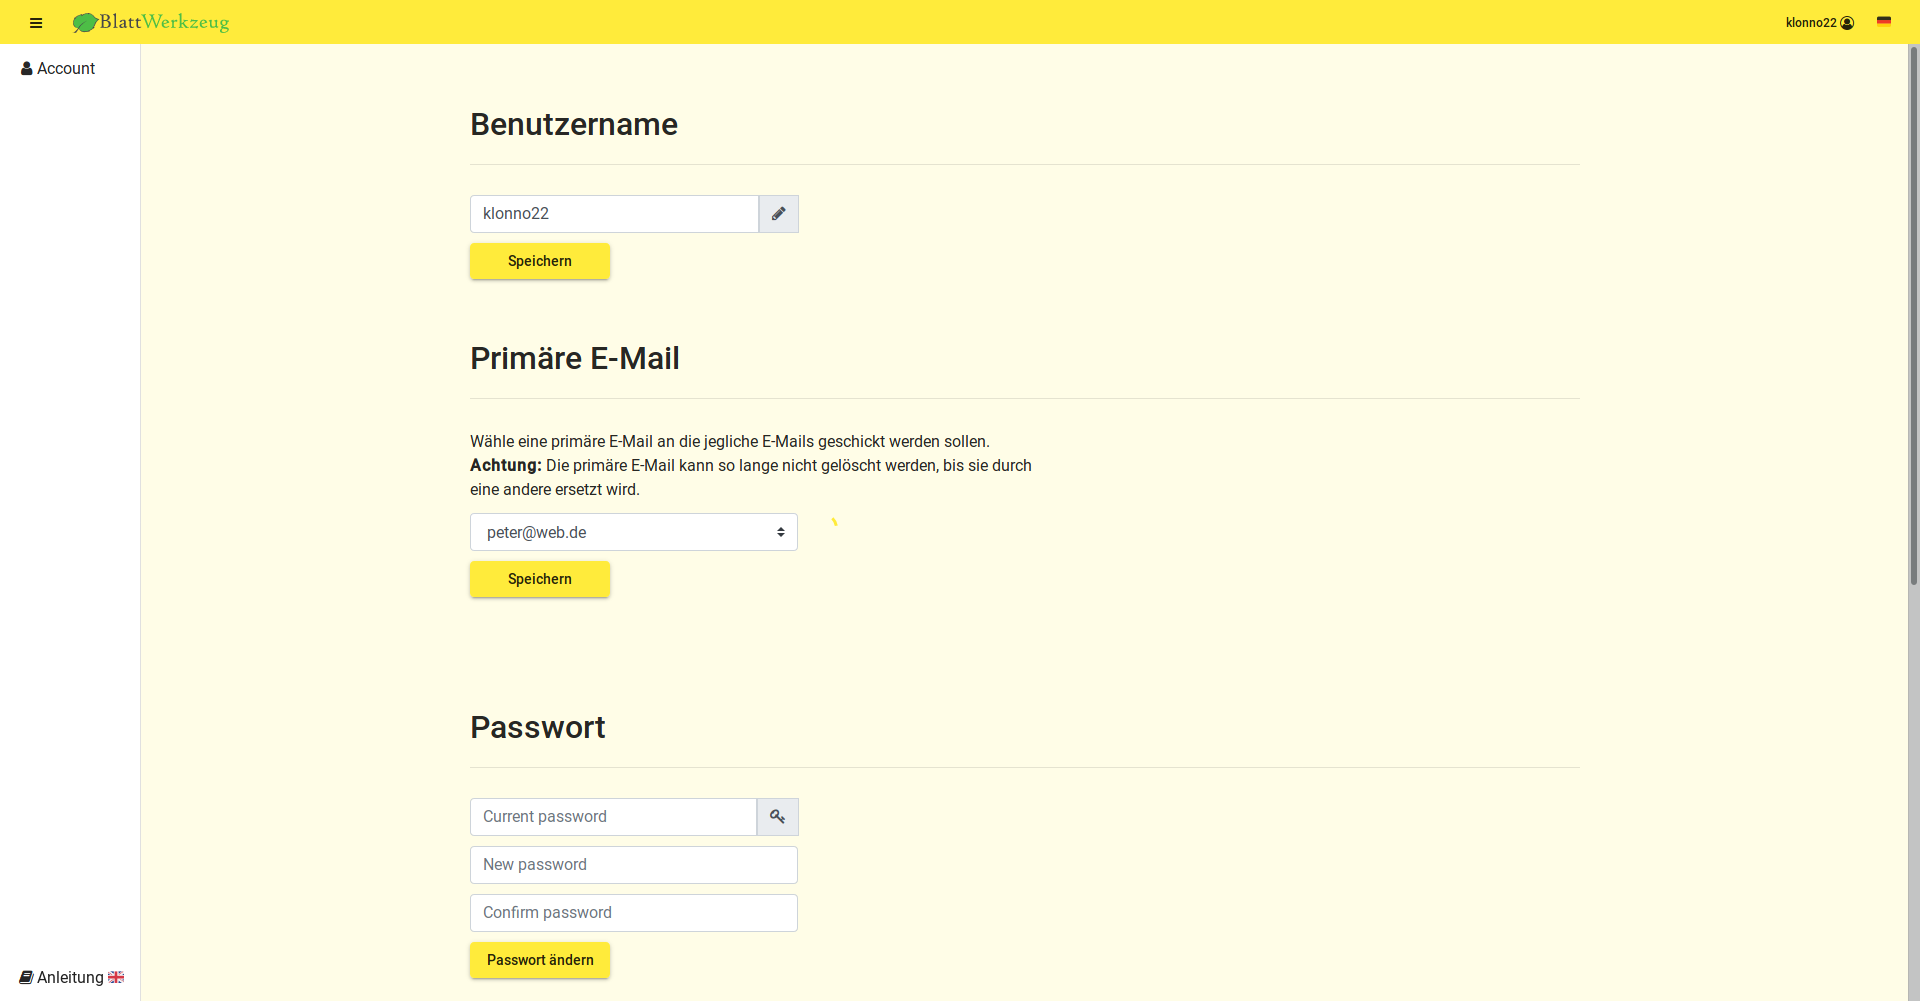
\includegraphics[width=\textwidth]{graphics/account-settings-1.png}
	\caption{Standart und erweiterte Ausführung eines validate-input}
	\label{fig:account_settings_1}
\end{figure}

\begin{figure}
	\centering
	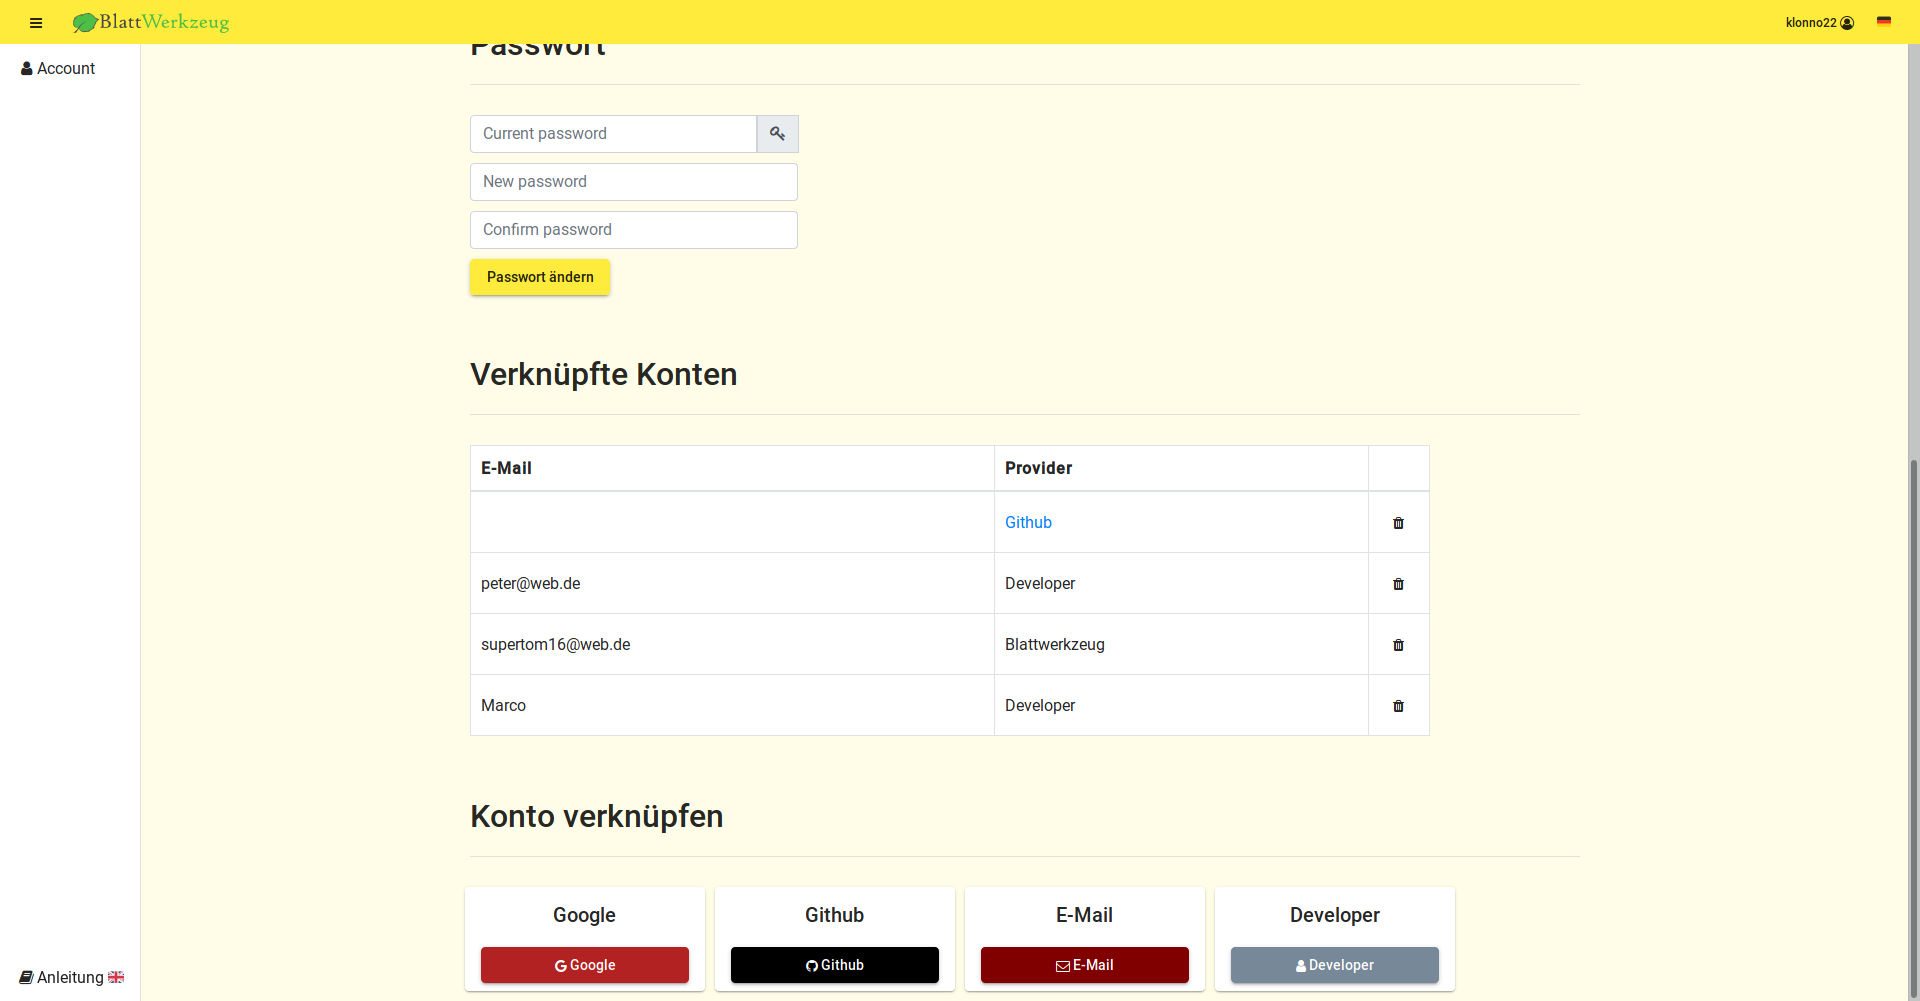
\includegraphics[width=\textwidth]{graphics/account-settings-2.png}
	\caption{Standart und erweiterte Ausführung eines validate-input}
	\label{fig:account_settings_2}
\end{figure}

\subsubsection{Wrapper-Komponenten}
\label{sec:client-wrapper-components}
Die Darstellung der Blattwerkzeug-Seite muss abhängig von den Rollen eines Benutzers sein. Hierfür ist es möglich die Unterteilung der einzelnen Codeabschnitte jeweils mit der Angular internen *If Direktive zu lösen. Eine weitere Möglichkeit wäre, die zu den Rollen angepassten Codeabschnitte jeweils in eigene Komponenten auszulagern. Ebenso ist es Möglich eine Wrapper-Komponente zu entwickeln, die dynamisch den Inhalt ihres Templates lädt und hierbei bedingt zwischen dem übermittelten Inhalt unterscheiden kann.

Das Nutzen der *If Direktive Angulars für jegliche Codeabschnitte, hat den Nachteil, dass erhöhte Coderedundanz vorkommt. Jede Komponente die Codeabschnitte abhängig von einer Rolle besitzt, müsste auf die jeweiligen Rollen eines Benuzers Zugriff haben. Dafür müsste in jede Komponente ein Service mit eingebunden werden, der die derzeitigen Rollen eines Benutzers an die Komponente ausliefert.

Die Unterteilung der einzelnen Codeabschnitte in eigene Komponenten hat den Nachteil das diese nicht flexibel sind. Eigene Komponenten würden sich stark auf die benötigte Rolle fokusieren. Sollte der Name dieser Rolle geändert werden, müsste nicht nur die Rollen-Abfrage verändert werden, sondern zusätzlich der jeweilige Name der Komponente.

Eine Wrapper-Komponente die dynamisch ihren Inhalt lädt und gleichzeitig bedingt auf den Inhalt achtet, verhindert erhöhte Coderedundanz und ermöglicht eine einfache Erweiterbarkeit oder Veränderung der Komponente. Aus diesen Gründen wurde sich für diese Methode entschieden.
\begin{description}
	\item[may\_perform]\hfill\\
	Bedienelemente, die von der jeweiligen Benutzerrolle abhängen, wie beispielsweise das Bedienelement zum Speichern eines Projektes, werden mittels may\_perform Wrapper-Komponente überprüft und dargestellt. Da es sich bei Projekten um Resourcen handelt, die nur bei spezifischer Berechtigung bearbeitet werden dürfen, müssen die Bedienelemente der jeweiligen Resource ausgeblendet werden. Sollten die Bedienelemente weiterhin dargestellt werden, kann dies zu einer schlechten User Experience, da ein Benutzer erst nach der Benutzung des Bedienelementes über eine unzureichende Berechtigung informiert wird. Damit eine Überprüfung serverseitig stattfinden kann, wurde sich vorerst mit den zu übermittelnden Daten beschäftigt. Für die Überprüfung der jeweiligen Funktion eines Bedienelementes, muss der Client die auf dem Server auszuführende Funktion angeben. Hierbei musste darauf geachtet werden, dass serverseitig nur Funktionen einer Policy ausgeführt werden können (Sektion \ref{sec:server-authorisation}). Desweiteren benötigt der Server die Informationen auf welcher Ressource diese Funktion ausgeführt werden soll. Sollte es sich bei der Überprüfung um eine spezifische Ressource handeln, muss ebenfalls die ID der Ressource übermittelt werden.
	
	\lstinputlisting[language=JavaScript, style=CodeView, caption=Interface der zu übermittelnden Daten, captionpos=b]{snippets/may-perform.ts}
	
	Die may-perform Daten wurden in eine Basisklasse und verschiedene abgeleitete Klassen unterteilt. Dabei beinhaltet die Basisklasse jegliche Daten, die Resourcen-übergreifend sind. Die abgeleiteten Klassen beinhalten spezialisierte Daten für eine Resource (Abbildung \ref{fig:client-data-pattern}). Der Service, der zum Aufruf dieser Daten injiziert wird, erstellt beim Aufruf einer Funktion, eine Instanz dieser Klasse. Ein Vorteil dieses Musters ist, dass die Struktur der Daten eindeutig ist, da die abgeleiteten Klassen jeweils einer Ressource entsprechen. Die Funktionen innerhalb des Services werden nach den jeweiligen Resourcen benannt. Daraus resultiert ein eindeutiges Aufruf-Muster, welches den Ressourcen-Namen gefolgt von der Aktion enhält (Listing \ref{lst:client-example_data_pattern}). 
	
	\begin{figure}
		\centering
		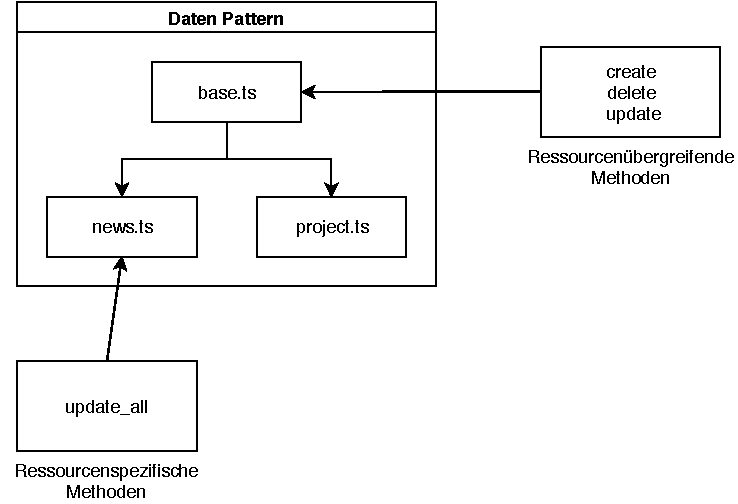
\includegraphics[width=\textwidth]{graphics/data-pattern.pdf}
		\caption{Struktur des Daten-Musters}
		\label{fig:client-data-pattern}
	\end{figure}

	\begin{minipage}{\linewidth}
		\lstinputlisting[language=JavaScript, style=CodeView, caption=Beispiel Aufruf zum erhalten der News-Daten, captionpos=b, label={lst:client-example_data_pattern}]{snippets/example_data_pattern.ts}
	\end{minipage}

	Schlussendlich wird ein Boolscher-Wert an den Client ausgeliefert. Sollte der Boolsche-Wert true zurückliefern, wird das Bedienelement dargestellt.
	
	\item[is-logged-in]\hfill\\
	Ein Besucher erhält  bei einem Aufruf der Blattwerkzeug-Seite Informationen über seinen derzeitigen Benutzer. Die übermittelten Informationen enthalten die Benuzter-Id, die Rollen, die primäre E-Mail und den Benutzernamen. Aus diesem Grund benötigen einige Bedienelemente keine serverseitige Berechtigungs-Abfrage. Das Nutzen  der may-perform Komponente wäre in diesem Fall eine überflüssige Maßname, da diese Bedienelemente ausschließlich auf eine statische Rolle geprüft werden.
	
	Die is-logged-in Wrapper-Komponente nutzt die vom Server übermittelten Rollen zur Überprüfung eines angemeldeten Benutzers. Ein angemeldeter Benutzer, wird clientseitig an seiner Rolle identifiziert. Hierfür werden die übermittelten Rollen auf eine guest Rolle geprüft. Das Vorhandensein einer guest Rolle, stellt einen unangemeldeten Benutzer dar. Die Darstellung eines umschlossenen HTML Codeabschnittes mittels is-logged-in hängt von dem derzeitigen Anmeldestatus eines Benutzers ab.  
\end{description}

\subsubsection{Routing-Guards}
\label{sec:routing-guards}
Derzeit ist das Navigieren auf jede Blattwerkzeug-Seite möglich. Routing Guards in Angular bieten die Möglichkeit das Navigieren einzuschränken. Hierfür stellt Angular verschiedene Typen an Routing Guards zur Verfügung. 

\begin{description}
	\item[CanActivate]\hfill\\
	Das CanActivate Interface von Angular wird genutzt um eine Bedingte Navigierung zu ermöglichen. Hierbei steht das CanActivate Interface für eine Überprüfung einer aktivierten Route. Eine Route gilt dann als aktiviert, wenn der Routing Guard mit dem CanActivate Interface einen Wahrheitswert zurückliefert. Der Fehlschlag eines CanActivate Routing Guards verhindert jedoch nicht das Laden von Routen gebudenen Modulen.
	\item[CanLoad]\hfill\\
	Das CanLoad Interface von Angular wird für das Bedingte Laden von Modulen verwendet. Im Gegensatz zum CanActivate Interface werden Routen gebudene Module, beim Fehlschlag eines CanLoad basierenden Routing Guards, nicht geladen.
\end{description}

Für die Einschränkung der Navigation auf Blattwerkzeug, wurden verschiedene Routing Guards erstellt.

\begin{description}
	\item[AdminGuard]\hfill\\
	Damit Bereiche wie beispielsweise der Adminbereich ausschließlich von Administratoren besucht werden können, wurde ein AdminGuard implementiert. Für die Überprüfung des AdminGuards werden die statischen Rollen eines Benutzers auf eine admin Rolle geprüft. Sollte dem derzeitigen Benutzer keine admin Rolle zugewiesen sein, wird dem Benutzer eine Fehlermeldung angezeigt. Die Fehlermeldung wurde mittels Asynchroner-Funktion und einem Dialog-Fenster implementiert. Das Dialog-Fenster bietet die Möglichkeit, mittels afterClosed Funktion, ein Observable als Rückgabewert festzulegen.
	
	Zitat:
	 \begin{quote}
		``Ein Observable ist die Repräsentation einer beliebigen Menge von Werten, die über eine beliebige Zeitdauer verteilt sein könnnen.``\footnote{\url{https://www.buschmais.de/wp-content/uploads/2019/01/01-2019-Java-aktuell_AUTOR_Michael-Ruttka_Einfuehrung-in-RxJS.pdf}}
	\end{quote}

	Das Schließen des Dialog-Fensters löst das zurückgegebene Observable aus. Sobald das Observable ausgelöst wurde, wird auf die Startseite zurück navigiert.
	
	\item[LoggedInGuard]\hfill\\
	Der LoggedInGuard ähnelt in seiner Funktionsweise dem AdminGuard. Allerdings wird dieser Routing Guard zur Überprüfung eines eingeloggten Benutzers verwendet. Die Einstellungen für Sicherheit und Login dürfen beispielsweise ausschließlich als angemeldeter Benutzer eingesehen werden. Sollte ein unangemeldeter Benutzer eine von einem LoggedInGuard geschützte Route besuchen, erhält dieser die Möglichkeit sich vorerst anzumelden. Da der LoggedInGuard sich ausschließlich im Dialog-Fenster und der zu überprüfenden Rolle von dem AdminGuard unterscheidet, wird die Implementierung nicht weiter erläutert.
	
	\item[MasterGuard]\hfill\\
	Bevor der AdminGuard oder der LoggedInGuard fehlschlägt, werden jeweils Dialog-Fenster geöffnet. Sollten mehrere Routing Guards für eine Route festgelegt werden, werden beim fehlschlagen der Routing Guards die Dialog-Fenster übereinander gelegt. Die Ursache dafür ist das, von Angular festgelegte, gleichzeitige Ausführen von Routing Guards. Aus diesem Grund muss ein Algorithmus zum ausführen nacheinander gefolgter Routing Guards implementiert werden. 
	
	Der MasterGuard implementiert einen Algorithmus zum ausführen nacheinander gefolgter Routing Guards. Hierfür werden die auszuführenden Routing Guards im data Objekt des Routes Typen hinterlegt. Sobald der MasterGuard aufgerufen wird, wird über die von Angular übergebene Route auf das data Objekt zugegriffen. Anschließend wird von jedem, im data Objekt enhaltenen, Routing Guard eine Instanz erstellt und die canActivate Methode aufgerufen. Sollte ein Routing Guard felschlagen, schlägt der Master Guard ebenfalls fehl.

\end{description}

%%% Local Variables:
%%% mode: latex
%%% TeX-master: "Tom - Thesis"
%%% End:

	\section{Fazit}
\label{sec:conclusion}

Ein Blick auf die im Anhang vorgestellten Projekte (\fullref{sec:project-examples}) zeigt, dass der Prototyp dem eingangs erwähnten Ziel\footnote{"`Mit dem Blattwerkzeug lassen sich gestützt durch \textit{Drag \& Drop-Editoren} für beliebige \texttt{SQLite}-Datenbanken \textit{Abfragen formulieren} und \textit{Oberflächen entwickeln}"', siehe Kapitel \fullref{sec:introduction}} durchaus gerecht wird: Zu praktisch beliebigen SQLite-Datenbanken können Abfragen und Oberflächen entwickelt werden.

Etwas detaillierter lässt sich der Grad des Erfolges einer Software vor allem am finalen Entwicklungsstand festmachen: Welcher prozentuale Anteil der angestrebten Funktionalität wurde erreicht? Daher muss sich der "`fertige Prototyp"' an den in Kapitel \fullref{sec:principles} formulierten Zielen messen lassen. Auch einige spätere Kapitel, insbesondere \fullref{sec:sql-subset}, lassen sich als ein recht umfassender Anforderungskatalog verstehen. Die formulierte Roadmap (siehe \fullref{sec:implementation-roadmap}) wurde bis auf den letzten Punkt "`Qulitätssicherung"' eingehalten. Eine Ausweitung der in Kapitel \fullref{sec:implementation-tests} beschriebenen Testmethodiken steht also ebenfalls noch aus.

Dieses vermeintlich objektive Kriterium der prozentualen Vollständigkeit berücksichtigt aber nur einen Teil der für Prototypen wie  \idename{} relevanten Ziele. Da in diesem Fall auf dem prototypischen Stand weiter aufgebaut werden soll, ist eine weitere Frage von Bedeutung: Kann man auf diesem Stand die Weiterentwicklung fortführen?

\subsection{Erreichte Ziele}

Der aktuelle Stand der Implementierung ist vor allem als ein Durchstich zu verstehen: Auch wenn es in fast jedem Teilbereich noch vereinzelt an Funktionalitäten fehlt, kann das Zusammenspiel dieser Systeme schon gut erprobt werden. Insbesondere bei der Verbindung der Datenbank mit der Oberfläche, sowohl lesend als auch schreibend, haben sich im Laufe der konkreten Implementierung noch einige unerwartete Stolpersteine aufgetan (\fullref{sec:unexpected-problems}). Das zugrundeliegende Fundament, also die internen und textuellen Darstellungen von \texttt{SQL} und \texttt{HTML}, sind aber stabil und darüber hinaus auch mächtiger, als der mit dem Drag \& Drop-Editor editierbare Stand.

Das Grundprinzip "`\textbf{Semantik vor Syntax}"' wurde erreicht, der Drag \& Drop-Editor schließt Syntaxfehler kategorisch aus. Sofern diese im kompilierten Quelltext doch auftreten, wäre das eindeutig ein Fehler in der Codegenerierung, nicht jedoch des Entwicklers. Bei Fehlermeldungen für erkannte Fehlersituationen gibt es jedoch noch Verbesserungspotenzial: Aktuell werden fehlerhafte Eingaben einfach zugelassen und dann erst im Nachhinein als Fehler markiert. An dieser Stelle wäre das im Prinzip angesprochene "`kontinuierliche Feedback"' vermutlich am besten mit einer eingebauten, kontextsensitiven Hilfe unterstützen. Diese könnte auf Fehler mit einer kurzen Erläuterung reagieren und dabei demonstrieren, wie die richtige Vorgehensweise wäre.

Ob die erstellbaren Seiten durch "`\textbf{praktisch vorzeigbare Ergebnisse motivieren}"', kann nur ein Test mit Probanden der Zielgruppe zeigen (siehe \fullref{sec:target-audience}). Ein Fortschritt gegenüber der nicht sonderlich hohen Hürde "`besser sein als Texteingaben in einer \texttt{SQL}-\texttt{IDE}"' ist aber durchaus zu erwarten.

Die "`\textbf{einfache Inbetriebnahme}"' ist vor allem eine Frage der Perspektive. Aus Sicht eines Schülers ist der Aufruf einer \texttt{URL} in der Tat einfach. Bisher hat \idename{} unter allen ad-hoc probierten Kombinationen aus Betriebssystemen (Windows, Mac\-OS, Linux) und Browsern (Firefox, Chrome, Edge) gut funktioniert. Für Lehrkräfte wird aktuell eine virtuelle Maschine bereitgestellt. Der Umgang mit dieser ist aufgrund des fehlenden Webinterfaces allerdings noch relativ unbequem.

Eine Notwendigkeit des Wechsels auf eine "`normale"' Desktopanwendung hat sich zu keinem Zeitpunkt ergeben. Das technische Fundament aus Ruby mit Sinatra und Typescript mit Angular 2 hat sich ebenso bewährt, wie die Entscheidung, den größten Teil der Logik im Client zu belassen. Der Betrieb von \idename{} ist nach der initialen Ladezeit fast vollständig frei von Verzögerungen. Die Möglichkeit der Entwicklung von Unit- und End-to-End-Tests fügt sich gut in den Entwicklungszyklus ein.

\subsection{Nicht erreichte Ziele}

Das Ziel einer "`\textbf{schrittweise komplexeren Benutzeroberfläche}"' wurde zunächst hinten angestellt, da es mit einem ausgearbeiteten Konzept einhergehen sollte. Kapitel \fullref{sec:sql-subset-ranks} untersucht zwar die möglichen Einschränkungen für \texttt{SQL}, geht aber nicht auf \texttt{HTML} oder die möglichen Auswirkungen auf das Zusammenspiel beider Systeme ein. Mit dem aktuell noch überschaubaren Funktionsumfang ist der akute Bedarf nach diesem spezifischen Grundprinzip allerdings auch noch nicht gegeben.

Zudem wurde das Ziel der "`\textbf{Fortführung der entwickelten Projekte}"' mit externen Programmen im Rahmen des Prototypen hinten angestellt. Zumindest die Unterstützung der Quelltext-Editoren sollte noch implementiert werden, bevor der Bedarf für einen Export überhaupt abgeschätzt werden kann.

Der Umfang der tatsächlich implementierten \texttt{SQL}-Funktionen ist noch nicht abgeschlossen. Zum jetzigen Zeitpunkt fehlen neben der Unterstützung der \texttt{AS}-Direktive im Editor (der Syntaxbaum unterstützt die Benennung bereits) vor allem Funktionen und Gruppierungen. Dieser Umstand schränkt die umsetzbaren Projekte empfindlich ein: Stünden diese Funktionen schon zur Verfügung, könnten zum Beispiel auch Webseiten für Sportvereine, inklusive der dynamischen Erzeugung von Tabellen, mit \idename{} umgesetzt werden.

Der Einsatz des Prototypen im Unterricht ist aktuell vor allem aufgrund der rudimentären Benutzerverwaltung nur schwer vorstellbar. Noch ist keine Registrierung von Benutzern implementiert, außerdem können Projekte nicht über die Webseite kopiert werden. Die Implementierung einer Benutzerverwaltung ist allerdings eine vor allem handwerkliche Aufgabe und wurde daher im Rahmen dieser Thesis nicht vorangetrieben.

Aber auch der Betrieb für Lehrkräfte gestaltet sich deutlich komplizierter als erwünscht: Die Notwendigkeit einer eigenen (Sub-)Domain ist keine triviale Hürde. Die Annahme "`man wird doch wohl mal auf dem Nameserver der Schuldomain einen Eintrag für \idename{} anlegen können"' hat sich zwar nicht als haltlos erwiesen, behindert die initiale Inbetriebnahme aber merklich.

\subsection{Weiterentwicklung}

Eine offene Frage bei der Weiterentwicklung von \idename{} ist die Wahl des Zeitpunkts, zu welchem die eigentliche Zielgruppe (sowie deren Lehrkräfte) in die Entwicklung mit einbezogen werden. Oder anders ausgedrückt: Es stellt sich die Frage nach dem minimalen Satz an implementierten Funktionen, mit denen man sinnvoll Feedback bei Lehrern und Schülern einholen kann.

Die folgende Aufzählung von offenen Baustellen gibt vor allem Anhaltspunkte, an welchen Stellen die prototypische Implementierung unvollständig ist. Diese Punkte sind dabei notwendig für einen tatsächlichen Einsatz im Unterricht, aber nicht zwingend hinreichend. Insbesondere die Erfüllung von weichen Kriterien, zum Beispiel eine umfassende Qualitätssicherung oder bessere Dokumentation für Schüler \& Lehrkräfte, werden nicht aufgeführt.

\begin{description}[noitemsep]
\item[Allgemein: Textuelle Editoren] \hfill\\
  Momentan begrenzen die Drag \& Drop-Editoren den Leistungsumfang ganz erheblich: Das interne Datenmodell ist hingegen darauf ausgelegt, auch textuelle Darstellungen "`blind"' entgegenzunehmen. Um Frust aufgrund von (noch?) nicht unterstützten Ideen zu vermeiden, sollten daher Texteditoren als "`Notausgang"' implementiert werden. Im Falle von \texttt{HTML} ist das über das spezielle Code-Bedienelement schon in Ansätzen möglich, für \texttt{SQL} hingegen noch überhaupt nicht.
  
\item[SQL: Unterstützung für Funktionen und \texttt{GROUP BY}] \hfill\\
  Ohne Aggregation von Daten lassen sich viele alltägliche Fragestellungen nicht beantworten. Glücklicherweise ist die eigentliche Implementierung nicht besonders aufwändig: Der Syntaxbaum ist darauf vorbereitet, für die Oberfläche ergeben sich keine bisher nicht schon gesehenen Anforderungen.
  
\item[SQL: Schemaeditor] \hfill\\
  Die Umsetzung eigener Ideen ist mit dem gegenwärtigen Stand faktisch nicht durchführbar, da es keine Möglichkeit gibt, das Datenbankschema über die Weboberfläche zu editieren. Eine Minimallösung wäre der einfache Upload von SQLite-Dateien, dann erfordert aber jede Anpassung des Schemas den Wechsel in ein externes Werkzeug.

  Die optimale Lösung wäre ein in \idename{} integrierter Schema-Editor. Mit diesem sollte man mindestens Tabellen und Spalten anlegen, umbenennen sowie löschen können. Aufwändig, aber sehr interessant wäre noch die Definition von Beziehungen.

\item[Seiten: Drag \& Drop für interpolierte Ausdrücke] \hfill\\
  Gegenwärtig müssen Liquid-Objekte unmittelbar in geschweiften Klammern im Quelltext notiert werden, es findet nicht einmal Syntax-Highlighting statt. Dieser Stand bricht daher nicht nur mit dem Drag \& Drop-Paradigma, er verwirrt auch mit schwer nachvollziehbaren Meldungen bei Syntaxfehlern. Folglich sollte in einer zukünftigen Version auch für diesen Bereich Drag \& Drop-Unterstützung durch \idename{} erfolgen.
  
\item[Seiten: Drag \& Drop für Kontrollstrukturen] \hfill\\
  Bisher ist der Entwickler darauf angewiesen, dass für Wiederholungen spezielle Bedienelemente wie die Datentabelle zur Verfügung gestellt werden, Verzweigungen lassen sich momentan außerhalb des \texttt{HTML}-Text-Elementes überhaupt nicht nutzen. Um diesem Umstand zu begegnen, sollten die Liquid-Tags \texttt{for} und \texttt{if} wie die vorhandenen Bedienelemente im Drag \& Drop-Editor repräsentiert werden können.  
\end{description}

Und abseits von den Details der Editoren für \texttt{HTML} und \texttt{SQL} ist auch noch eine Grundsatzentscheidung zu treffen: Die Form, in der \idename{} Lehrkräften zugänglich gemacht werden soll. Das Feedback aus informellen Gesprächen gibt zumindest Anlass, die eingangs formulierte Prämisse "`jeder Lehrer stellt halt einen Server für seine Klassen bereit"' erneut zu hinterfragen. Ein dazu häufig formulierter Kritikpunkt lässt sich mit "`Immerhin wird Scratch auch einfach so im Web angeboten"' zusammenfassen. Dieser Ansatz wäre natürlich auch denkbar, eine solche Entscheidung hat aber enorme Tragweite und wirft viele Fragen auf: Kann die Anmeldung über einen Dienst der Schulen erfolgen? Was für Auswirkugen hat das auf interessierte Schülerinnen ohne eine Schule im Hintergrund? Sollen die Schüler unterschiedlicher Schulen miteinander interagieren können? Wer haftet bei Verstößen gegen das Urheberrecht? Wer bezahlt den Betrieb der notwendigen Server? All diese (und vermutlich noch weitere) Fragen werden im Falle einer Umstellung zu klären sein.




%%% Local Variables:
%%% mode: latex
%%% TeX-master: "thesis"
%%% End:


\end{document}
%%% Local Variables:
%%% mode: latex
%%% TeX-engine: xetex
%%% TeX-master: t
%%% End:
